\documentclass[t]{beamer}
\usepackage{physics}
\usepackage{amsmath}
\usepackage{tikz}
\usepackage{mathdots}
\usepackage{yhmath}
\usepackage{cancel}
\usepackage{color}
\usepackage{siunitx}
\usepackage{array}
\usepackage{multirow}
\usepackage{amssymb}
\usepackage{mathtools}
\usepackage{textcomp, gensymb}
\usepackage{tabularx}
\usepackage{extarrows}
\usepackage{booktabs}
\usetikzlibrary{fadings}
\usetikzlibrary{patterns}
\usetikzlibrary{shadows.blur}
\usetikzlibrary{shapes}
\usepackage[style=verbose,backend=bibtex]{biblatex}
\addbibresource{boltzmann.bib}
\usepackage{listings}
\usepackage{hyperref}

\newcommand{\pair}[1]{\langle #1 \rangle}
\DeclareMathOperator{\ee}{e}
\DeclareMathOperator{\ii}{i}
\DeclareMathOperator{\timeorder}{\mathcal{T}}

\newcommand{\concept}[1]{\textbf{#1}}

%region Theme
\usetheme{Madrid}

% Show section in foot
\makeatletter
\setbeamertemplate{footline}
{
  \leavevmode%
  \hbox{%
  \begin{beamercolorbox}[wd=.333333\paperwidth,ht=2.25ex,dp=1ex,center]{author in head/foot}%
    \usebeamerfont{author in head/foot}\insertauthor
  \end{beamercolorbox}%
  \begin{beamercolorbox}[wd=.333333\paperwidth,ht=2.25ex,dp=1ex,center]{title in head/foot}%
    \usebeamerfont{title in head/foot}\insertsection
  \end{beamercolorbox}%
  \begin{beamercolorbox}[wd=.333333\paperwidth,ht=2.25ex,dp=1ex,right]{date in head/foot}%
    \usebeamerfont{date in head/foot}\insertshortdate{}\hspace*{2em}
    \insertframenumber{} / \inserttotalframenumber\hspace*{2ex} 
  \end{beamercolorbox}}%
  \vskip0pt%
}
\makeatother

%endregion

%Information to be included in the title page:
\title{Time-dependent adiabatic $GW$}
\author{Jinyuan Wu}

\begin{document}

\maketitle

\begin{frame}
\frametitle{Table of content}

\tableofcontents    

\end{frame}

\section{Overview}

\begin{frame}
\frametitle{Relation between formalisms}

\begin{center}
    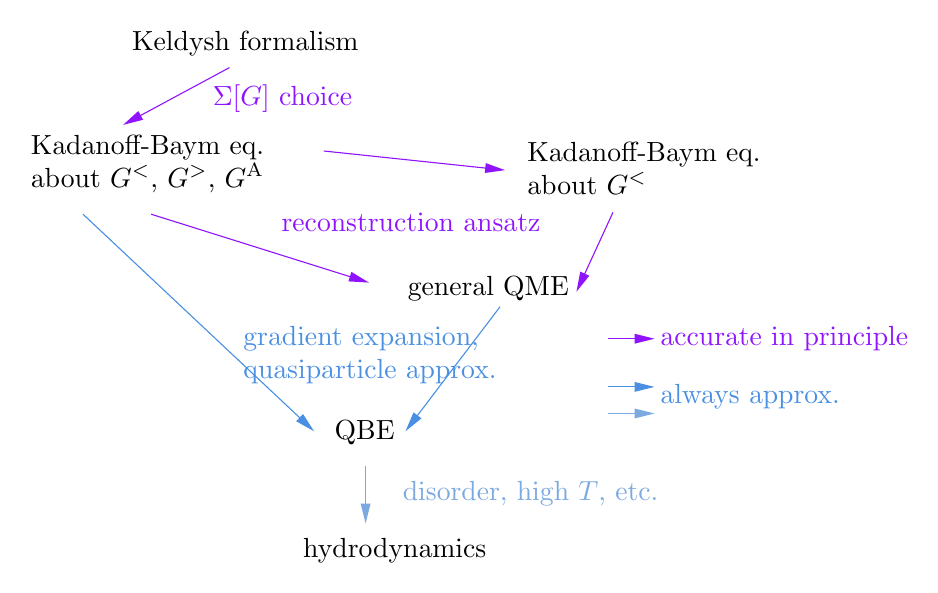
\begin{tikzpicture}[x=0.75pt,y=0.75pt,yscale=-0.8,xscale=0.8]
    %uncomment if require: \path (0,403); %set diagram left start at 0, and has height of 403
    
    %Straight Lines [id:da3574677469464902] 
    \draw [color={rgb, 255:red, 144; green, 19; blue, 254 }  ,draw opacity=1 ]   (226.17,66.27) -- (163.93,99.79) ;
    \draw [shift={(162.17,100.74)}, rotate = 331.69] [fill={rgb, 255:red, 144; green, 19; blue, 254 }  ,fill opacity=1 ][line width=0.08]  [draw opacity=0] (12,-3) -- (0,0) -- (12,3) -- cycle    ;
    %Straight Lines [id:da6278234902971178] 
    \draw [color={rgb, 255:red, 144; green, 19; blue, 254 }  ,draw opacity=1 ]   (179,154.55) -- (308.26,195.14) ;
    \draw [shift={(310.17,195.74)}, rotate = 197.43] [fill={rgb, 255:red, 144; green, 19; blue, 254 }  ,fill opacity=1 ][line width=0.08]  [draw opacity=0] (12,-3) -- (0,0) -- (12,3) -- cycle    ;
    %Straight Lines [id:da8214266493222495] 
    \draw [color={rgb, 255:red, 74; green, 144; blue, 226 }  ,draw opacity=1 ]   (138,154.55) -- (275.71,283.9) ;
    \draw [shift={(277.17,285.27)}, rotate = 223.21] [fill={rgb, 255:red, 74; green, 144; blue, 226 }  ,fill opacity=1 ][line width=0.08]  [draw opacity=0] (12,-3) -- (0,0) -- (12,3) -- cycle    ;
    %Straight Lines [id:da5242918677536943] 
    \draw [color={rgb, 255:red, 74; green, 144; blue, 226 }  ,draw opacity=1 ]   (389.17,210.27) -- (333.38,283.68) ;
    \draw [shift={(332.17,285.27)}, rotate = 307.23] [fill={rgb, 255:red, 74; green, 144; blue, 226 }  ,fill opacity=1 ][line width=0.08]  [draw opacity=0] (12,-3) -- (0,0) -- (12,3) -- cycle    ;
    %Straight Lines [id:da6748656000657882] 
    \draw [color={rgb, 255:red, 124; green, 170; blue, 224 }  ,draw opacity=1 ]   (308.17,306.27) -- (308.17,338.8) ;
    \draw [shift={(308.17,340.8)}, rotate = 270] [fill={rgb, 255:red, 124; green, 170; blue, 224 }  ,fill opacity=1 ][line width=0.08]  [draw opacity=0] (12,-3) -- (0,0) -- (12,3) -- cycle    ;
    %Straight Lines [id:da1182191617400088] 
    \draw [color={rgb, 255:red, 144; green, 19; blue, 254 }  ,draw opacity=1 ]   (283,116.49) -- (390.18,127.8) ;
    \draw [shift={(392.17,128.01)}, rotate = 186.02] [fill={rgb, 255:red, 144; green, 19; blue, 254 }  ,fill opacity=1 ][line width=0.08]  [draw opacity=0] (12,-3) -- (0,0) -- (12,3) -- cycle    ;
    %Straight Lines [id:da3233811707634906] 
    \draw [color={rgb, 255:red, 144; green, 19; blue, 254 }  ,draw opacity=1 ]   (457.17,153.41) -- (436,199.45) ;
    \draw [shift={(435.17,201.27)}, rotate = 294.68] [fill={rgb, 255:red, 144; green, 19; blue, 254 }  ,fill opacity=1 ][line width=0.08]  [draw opacity=0] (12,-3) -- (0,0) -- (12,3) -- cycle    ;
    %Straight Lines [id:da7080246790835758] 
    \draw [color={rgb, 255:red, 144; green, 19; blue, 254 }  ,draw opacity=1 ]   (454,229.55) -- (480.17,229.55) ;
    \draw [shift={(482.17,229.55)}, rotate = 180] [fill={rgb, 255:red, 144; green, 19; blue, 254 }  ,fill opacity=1 ][line width=0.08]  [draw opacity=0] (12,-3) -- (0,0) -- (12,3) -- cycle    ;
    %Straight Lines [id:da3562948391141818] 
    \draw [color={rgb, 255:red, 74; green, 144; blue, 226 }  ,draw opacity=1 ]   (454,258.55) -- (480.17,258.55) ;
    \draw [shift={(482.17,258.55)}, rotate = 180] [fill={rgb, 255:red, 74; green, 144; blue, 226 }  ,fill opacity=1 ][line width=0.08]  [draw opacity=0] (12,-3) -- (0,0) -- (12,3) -- cycle    ;
    %Straight Lines [id:da28735661944331214] 
    \draw [color={rgb, 255:red, 124; green, 170; blue, 224 }  ,draw opacity=1 ]   (454,274.55) -- (480.17,274.55) ;
    \draw [shift={(482.17,274.55)}, rotate = 180] [fill={rgb, 255:red, 124; green, 170; blue, 224 }  ,fill opacity=1 ][line width=0.08]  [draw opacity=0] (12,-3) -- (0,0) -- (12,3) -- cycle    ;
    
    % Text Node
    \draw (166,42.55) node [anchor=north west][inner sep=0.75pt]   [align=left] {Keldysh formalism};
    % Text Node
    \draw (258.1,84.99) node  [color={rgb, 255:red, 144; green, 19; blue, 254 }  ,opacity=1 ] [align=left] {$\displaystyle \Sigma [ G]$ choice};
    % Text Node
    \draw (105,105.55) node [anchor=north west][inner sep=0.75pt]   [align=left] {Kadanoff-Baym eq.\\about $\displaystyle G^{< }$, $\displaystyle G^{ >}$, $\displaystyle G^{\text{A}}$};
    % Text Node
    \draw (256,152.55) node [anchor=north west][inner sep=0.75pt]  [color={rgb, 255:red, 144; green, 19; blue, 254 }  ,opacity=1 ] [align=left] {reconstruction ansatz};
    % Text Node
    \draw (332,190.55) node [anchor=north west][inner sep=0.75pt]   [align=left] {general QME};
    % Text Node
    \draw (233,220.55) node [anchor=north west][inner sep=0.75pt]  [color={rgb, 255:red, 74; green, 144; blue, 226 }  ,opacity=1 ] [align=left] {gradient expansion,\\quasiparticle approx.};
    % Text Node
    \draw (288,277.55) node [anchor=north west][inner sep=0.75pt]   [align=left] {QBE};
    % Text Node
    \draw (329,314) node [anchor=north west][inner sep=0.75pt]  [color={rgb, 255:red, 124; green, 170; blue, 224 }  ,opacity=1 ] [align=left] {disorder, high $\displaystyle T$, etc.};
    % Text Node
    \draw (269,348) node [anchor=north west][inner sep=0.75pt]   [align=left] {hydrodynamics};
    % Text Node
    \draw (404,109.55) node [anchor=north west][inner sep=0.75pt]   [align=left] {Kadanoff-Baym eq.\\about $\displaystyle G^{< }$};
    % Text Node
    \draw (484.17,229.55) node [anchor=west] [inner sep=0.75pt]  [color={rgb, 255:red, 144; green, 19; blue, 254 }  ,opacity=1 ] [align=left] {accurate in principle};
    % Text Node
    \draw (484.17,264.55) node [anchor=west] [inner sep=0.75pt]  [color={rgb, 255:red, 74; green, 144; blue, 226}  ,opacity=1 ] [align=left] {always approx.};
    
    
    \end{tikzpicture}
    
\end{center}    

\end{frame}

\section{Kadanoff-Baym equations}

\begin{frame}
\frametitle{Non-equilibrium Green function}

\textbf{Motivation} 

\begin{equation}
    \expval*{A} = \expval*{S^{-1} \timeorder_t ( S A_{\text{I}}(t) )}, \quad S = U(\infty, -\infty)
\end{equation}
Non-equilibrium state: not pure; contains excited state components;

$\ket*{\Psi_n}$ is excited state $\Rightarrow$ $S \ket*{\Psi_n} \neq \ee^{\ii \alpha} \ket*{\Psi_n}$
$\Rightarrow$ we can't peel the $S^{-1}$ off!!

\vspace{0.5cm}

\textbf{Solution} Four (instead of one) types of propagators: (note $S^{-1}$ is \emph{anti}-time ordered)

\begin{center}
    \small
    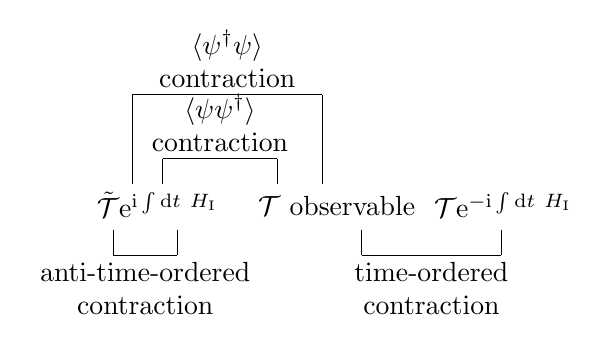
\begin{tikzpicture}[x=0.75pt,y=0.75pt,yscale=-0.7,xscale=0.7]
    %uncomment if require: \path (0,300); %set diagram left start at 0, and has height of 300
    
    %Straight Lines [id:da3326778841678064] 
    \draw    (135,167) -- (135,184.6) ;
    %Straight Lines [id:da14207491665960603] 
    \draw    (179,167) -- (179,184.6) ;
    %Straight Lines [id:da9585241583566635] 
    \draw    (135,184.6) -- (179,184.6) ;
    %Straight Lines [id:da5708657905713688] 
    \draw    (306,167) -- (306,184.6) ;
    %Straight Lines [id:da9177451110065487] 
    \draw    (402,167) -- (402,184.6) ;
    %Straight Lines [id:da6223566418192004] 
    \draw    (306,184.6) -- (402,184.6) ;
    %Straight Lines [id:da8688775028052254] 
    \draw    (169,118.4) -- (169,136) ;
    %Straight Lines [id:da16336389755134917] 
    \draw    (248,118.4) -- (248,136) ;
    %Straight Lines [id:da09889506498736633] 
    \draw    (169,118.4) -- (248,118.4) ;
    %Straight Lines [id:da5570498155343657] 
    \draw    (148,74.3) -- (148,136) ;
    %Straight Lines [id:da7392127913533113] 
    \draw    (148,74.3) -- (279,74.3) ;
    %Straight Lines [id:da826347580065202] 
    \draw    (279,74.3) -- (279,136) ;
    
    % Text Node
    \draw (122,139.5) node [anchor=north west][inner sep=0.75pt]    {$\tilde{\mathcal{T}} \mathrm{e}^{\mathrm{i}\int \mathrm{d} t\ H_{\text{I}}}$};
    % Text Node
    \draw (233,142) node [anchor=north west][inner sep=0.75pt]   [align=left] {$\displaystyle \mathcal{T}$ observable};
    % Text Node
    \draw (354,139.5) node [anchor=north west][inner sep=0.75pt]    {$\mathcal{T}\mathrm{e}^{-\mathrm{i}\int \mathrm{d} t\ H_{\text{I}}}$};
    % Text Node
    \draw (157,187.6) node [anchor=north] [inner sep=0.75pt]   [align=left] {\begin{minipage}[lt]{83.43pt}\setlength\topsep{0pt}
    \begin{center}
    anti-time-ordered \\contraction
    \end{center}
    
    \end{minipage}};
    % Text Node
    \draw (354,187.6) node [anchor=north] [inner sep=0.75pt]   [align=left] {\begin{minipage}[lt]{62.78pt}\setlength\topsep{0pt}
    \begin{center}
    time-ordered \\contraction
    \end{center}
    
    \end{minipage}};
    % Text Node
    \draw (208.5,115.4) node [anchor=south] [inner sep=0.75pt]   [align=left] {\begin{minipage}[lt]{52.85pt}\setlength\topsep{0pt}
    \begin{center}
    $\displaystyle \langle \psi \psi ^{\dagger } \rangle $\\contraction
    \end{center}
    
    \end{minipage}};
    % Text Node
    \draw (213.5,71.3) node [anchor=south] [inner sep=0.75pt]   [align=left] {\begin{minipage}[lt]{52.85pt}\setlength\topsep{0pt}
    \begin{center}
    $\displaystyle \langle \psi ^{\dagger } \psi \rangle $\\contraction
    \end{center}
    
    \end{minipage}};
    
    
    \end{tikzpicture}
        
\end{center}

\end{frame}

\begin{frame}
\frametitle{Keldysh formalism}

\textbf{Four types of (fermionic) propagators}

\begin{equation}
    \begin{aligned}
        \ii G^{--} &= \ii G^{\text{c}} = \expval*{\timeorder \psi_1 \psi_2^\dagger}, \quad 
        \ii G^{++} = \ii G^{\text{a}} = \expval*{\tilde{\timeorder} \psi_1 \psi_2^\dagger}, \\
        \ii G^{+-} &= \ii G^{>} = \expval*{\psi_1 \psi_2^\dagger},   \quad 
        \ii G^{-+} = \ii G^{<} = - \expval*{\psi_2^\dagger \psi_1}.
    \end{aligned}
\end{equation}    

\vspace{0.5cm}

\textbf{Diagrams} 

\begin{center}
    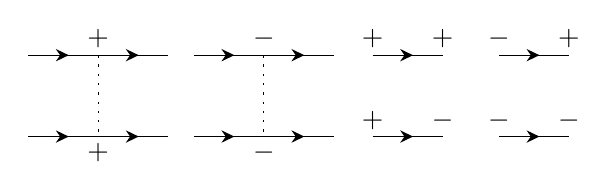
\begin{tikzpicture}[x=0.75pt,y=0.75pt,yscale=-0.7,xscale=0.7]
    %uncomment if require: \path (0,300); %set diagram left start at 0, and has height of 300
    
    %Straight Lines [id:da8169580565348766] 
    \draw    (35,78) -- (83.17,78) ;
    \draw [shift={(62.88,78)}, rotate = 180] [fill={rgb, 255:red, 0; green, 0; blue, 0 }  ][line width=0.08]  [draw opacity=0] (8.93,-4.29) -- (0,0) -- (8.93,4.29) -- (5.93,0) -- cycle    ;
    %Straight Lines [id:da9357207883622545] 
    \draw    (83.17,78) -- (131.33,78) ;
    \draw [shift={(111.05,78)}, rotate = 180] [fill={rgb, 255:red, 0; green, 0; blue, 0 }  ][line width=0.08]  [draw opacity=0] (8.93,-4.29) -- (0,0) -- (8.93,4.29) -- (5.93,0) -- cycle    ;
    %Straight Lines [id:da48155815853606776] 
    \draw    (35,134) -- (83.17,134) ;
    \draw [shift={(62.88,134)}, rotate = 180] [fill={rgb, 255:red, 0; green, 0; blue, 0 }  ][line width=0.08]  [draw opacity=0] (8.93,-4.29) -- (0,0) -- (8.93,4.29) -- (5.93,0) -- cycle    ;
    %Straight Lines [id:da7480670839969836] 
    \draw    (83.17,134) -- (131.33,134) ;
    \draw [shift={(111.05,134)}, rotate = 180] [fill={rgb, 255:red, 0; green, 0; blue, 0 }  ][line width=0.08]  [draw opacity=0] (8.93,-4.29) -- (0,0) -- (8.93,4.29) -- (5.93,0) -- cycle    ;
    %Straight Lines [id:da4153723089787493] 
    \draw  [dash pattern={on 0.84pt off 2.51pt}]  (83.17,78) -- (83.17,134) ;
    %Straight Lines [id:da9154821765962851] 
    \draw    (149,78) -- (197.17,78) ;
    \draw [shift={(176.88,78)}, rotate = 180] [fill={rgb, 255:red, 0; green, 0; blue, 0 }  ][line width=0.08]  [draw opacity=0] (8.93,-4.29) -- (0,0) -- (8.93,4.29) -- (5.93,0) -- cycle    ;
    %Straight Lines [id:da3027826223354886] 
    \draw    (197.17,78) -- (245.33,78) ;
    \draw [shift={(225.05,78)}, rotate = 180] [fill={rgb, 255:red, 0; green, 0; blue, 0 }  ][line width=0.08]  [draw opacity=0] (8.93,-4.29) -- (0,0) -- (8.93,4.29) -- (5.93,0) -- cycle    ;
    %Straight Lines [id:da1521558171041284] 
    \draw    (149,134) -- (197.17,134) ;
    \draw [shift={(176.88,134)}, rotate = 180] [fill={rgb, 255:red, 0; green, 0; blue, 0 }  ][line width=0.08]  [draw opacity=0] (8.93,-4.29) -- (0,0) -- (8.93,4.29) -- (5.93,0) -- cycle    ;
    %Straight Lines [id:da015084792241701894] 
    \draw    (197.17,134) -- (245.33,134) ;
    \draw [shift={(225.05,134)}, rotate = 180] [fill={rgb, 255:red, 0; green, 0; blue, 0 }  ][line width=0.08]  [draw opacity=0] (8.93,-4.29) -- (0,0) -- (8.93,4.29) -- (5.93,0) -- cycle    ;
    %Straight Lines [id:da8317921095867193] 
    \draw  [dash pattern={on 0.84pt off 2.51pt}]  (197.17,78) -- (197.17,134) ;
    %Straight Lines [id:da7041708770117445] 
    \draw    (272,78) -- (320.17,78) ;
    \draw [shift={(299.88,78)}, rotate = 180] [fill={rgb, 255:red, 0; green, 0; blue, 0 }  ][line width=0.08]  [draw opacity=0] (8.93,-4.29) -- (0,0) -- (8.93,4.29) -- (5.93,0) -- cycle    ;
    %Straight Lines [id:da24010158572243] 
    \draw    (272,134) -- (320.17,134) ;
    \draw [shift={(299.88,134)}, rotate = 180] [fill={rgb, 255:red, 0; green, 0; blue, 0 }  ][line width=0.08]  [draw opacity=0] (8.93,-4.29) -- (0,0) -- (8.93,4.29) -- (5.93,0) -- cycle    ;
    %Straight Lines [id:da3015830145357803] 
    \draw    (359,78) -- (407.17,78) ;
    \draw [shift={(386.88,78)}, rotate = 180] [fill={rgb, 255:red, 0; green, 0; blue, 0 }  ][line width=0.08]  [draw opacity=0] (8.93,-4.29) -- (0,0) -- (8.93,4.29) -- (5.93,0) -- cycle    ;
    %Straight Lines [id:da24391779212824316] 
    \draw    (359,134) -- (407.17,134) ;
    \draw [shift={(386.88,134)}, rotate = 180] [fill={rgb, 255:red, 0; green, 0; blue, 0 }  ][line width=0.08]  [draw opacity=0] (8.93,-4.29) -- (0,0) -- (8.93,4.29) -- (5.93,0) -- cycle    ;
    
    % Text Node
    \draw (83.17,75) node [anchor=south] [inner sep=0.75pt]   [align=left] {$+$};
    % Text Node
    \draw (83.17,137) node [anchor=north] [inner sep=0.75pt]   [align=left] {$+$};
    % Text Node
    \draw (197.17,75) node [anchor=south] [inner sep=0.75pt]   [align=left] {$-$};
    % Text Node
    \draw (197.17,137) node [anchor=north] [inner sep=0.75pt]   [align=left] {$-$};
    % Text Node
    \draw (272,75) node [anchor=south] [inner sep=0.75pt]   [align=left] {$+$};
    % Text Node
    \draw (320.17,75) node [anchor=south] [inner sep=0.75pt]   [align=left] {$+$};
    % Text Node
    \draw (272,131) node [anchor=south] [inner sep=0.75pt]   [align=left] {$+$};
    % Text Node
    \draw (320.17,131) node [anchor=south] [inner sep=0.75pt]   [align=left] {$-$};
    % Text Node
    \draw (359,75) node [anchor=south] [inner sep=0.75pt]   [align=left] {$-$};
    % Text Node
    \draw (407.17,75) node [anchor=south] [inner sep=0.75pt]   [align=left] {$+$};
    % Text Node
    \draw (359,131) node [anchor=south] [inner sep=0.75pt]   [align=left] {$-$};
    % Text Node
    \draw (407.17,131) node [anchor=south] [inner sep=0.75pt]   [align=left] {$-$};
    
    
    \end{tikzpicture}
    
\end{center}

\textbf{Self-energy} 

\begin{equation}
    G = \pmqty{
        G^{--} & G^{-+} \\ 
        G^{+-} & G^{++}
    }   , \quad 
    \Sigma = \pmqty{
        \Sigma^{--} & \Sigma^{-+} \\ 
        \Sigma^{+-} & \Sigma^{++}
    } , \quad 
    G = G_0 + G_0 \Sigma G.
\end{equation}

\end{frame}

\begin{frame}
\frametitle{Alternative formulation: Keldysh contour}

\textbf{Keldysh contour} The information in the $G$ matrix can be alternatively stored 
in a time-ordered Green function on \emph{Keldysh contour}

\begin{center}
    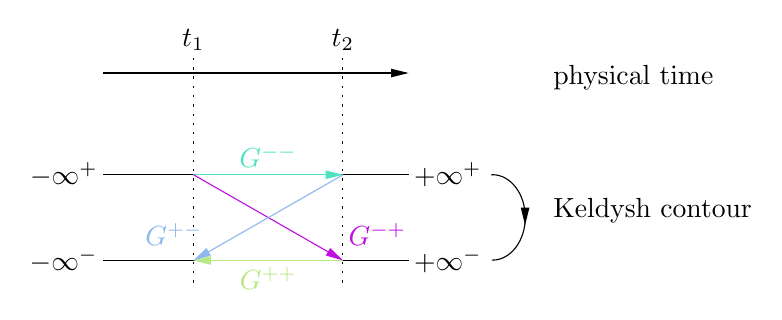
\begin{tikzpicture}[x=0.75pt,y=0.75pt,yscale=-0.7,xscale=0.7]
    %uncomment if require: \path (0,300); %set diagram left start at 0, and has height of 300
    
    %Straight Lines [id:da9923247639127166] 
    \draw    (144,152) -- (354.17,152) ;
    %Straight Lines [id:da5829772718809481] 
    \draw    (144,211) -- (354.17,211) ;
    %Straight Lines [id:da04548734740797422] 
    \draw  [dash pattern={on 0.84pt off 2.51pt}]  (206,71.6) -- (206,229) ;
    %Straight Lines [id:da1610984974972618] 
    \draw  [dash pattern={on 0.84pt off 2.51pt}]  (309,71.6) -- (309,229) ;
    %Straight Lines [id:da04350669910867855] 
    \draw    (144,82) -- (352.17,82) ;
    \draw [shift={(354.17,82)}, rotate = 180] [fill={rgb, 255:red, 0; green, 0; blue, 0 }  ][line width=0.08]  [draw opacity=0] (12,-3) -- (0,0) -- (12,3) -- cycle    ;
    %Straight Lines [id:da9269008755131121] 
    \draw [color={rgb, 255:red, 80; green, 227; blue, 194 }  ,draw opacity=1 ]   (206.17,152) -- (307.17,152) ;
    \draw [shift={(309.17,152)}, rotate = 180] [fill={rgb, 255:red, 80; green, 227; blue, 194 }  ,fill opacity=1 ][line width=0.08]  [draw opacity=0] (12,-3) -- (0,0) -- (12,3) -- cycle    ;
    %Straight Lines [id:da9541927407052295] 
    \draw [color={rgb, 255:red, 184; green, 233; blue, 134 }  ,draw opacity=1 ]   (208.17,211) -- (309.17,211) ;
    \draw [shift={(206.17,211)}, rotate = 0] [fill={rgb, 255:red, 184; green, 233; blue, 134 }  ,fill opacity=1 ][line width=0.08]  [draw opacity=0] (12,-3) -- (0,0) -- (12,3) -- cycle    ;
    %Straight Lines [id:da8455403205757837] 
    \draw [color={rgb, 255:red, 189; green, 16; blue, 224 }  ,draw opacity=1 ]   (206.17,152) -- (307.43,210.01) ;
    \draw [shift={(309.17,211)}, rotate = 209.8] [fill={rgb, 255:red, 189; green, 16; blue, 224 }  ,fill opacity=1 ][line width=0.08]  [draw opacity=0] (12,-3) -- (0,0) -- (12,3) -- cycle    ;
    %Straight Lines [id:da6613881717892212] 
    \draw [color={rgb, 255:red, 141; green, 183; blue, 237 }  ,draw opacity=1 ]   (309.17,152) -- (207.9,210.01) ;
    \draw [shift={(206.17,211)}, rotate = 330.2] [fill={rgb, 255:red, 141; green, 183; blue, 237 }  ,fill opacity=1 ][line width=0.08]  [draw opacity=0] (12,-3) -- (0,0) -- (12,3) -- cycle    ;
    %Shape: Arc [id:dp9263560588014466] 
    \draw  [draw opacity=0] (411.17,152) .. controls (411.43,151.99) and (411.69,151.98) .. (411.95,151.98) .. controls (424.42,151.98) and (434.53,165.14) .. (434.53,181.37) .. controls (434.53,197.6) and (424.42,210.76) .. (411.95,210.76) .. controls (411.84,210.76) and (411.73,210.76) .. (411.62,210.76) -- (411.95,181.37) -- cycle ; \draw   (411.17,152) .. controls (411.43,151.99) and (411.69,151.98) .. (411.95,151.98) .. controls (424.42,151.98) and (434.53,165.14) .. (434.53,181.37) .. controls (434.53,197.6) and (424.42,210.76) .. (411.95,210.76) .. controls (411.84,210.76) and (411.73,210.76) .. (411.62,210.76) ;  
    %Straight Lines [id:da9478596817855973] 
    \draw    (434.42,181.77) -- (434.42,184.6) ;
    \draw [shift={(434.42,186.6)}, rotate = 270] [fill={rgb, 255:red, 0; green, 0; blue, 0 }  ][line width=0.08]  [draw opacity=0] (12,-3) -- (0,0) -- (12,3) -- cycle    ;
    
    % Text Node
    \draw (142,152) node [anchor=east] [inner sep=0.75pt]    {$-\infty ^{+}$};
    % Text Node
    \draw (142,211) node [anchor=east] [inner sep=0.75pt]    {$-\infty ^{-}$};
    % Text Node
    \draw (356.17,152) node [anchor=west] [inner sep=0.75pt]    {$+\infty ^{+}$};
    % Text Node
    \draw (356.17,211) node [anchor=west] [inner sep=0.75pt]    {$+\infty ^{-}$};
    % Text Node
    \draw (452,176.5) node [anchor=west] [inner sep=0.75pt]   [align=left] {Keldysh contour};
    % Text Node
    \draw (206,68.6) node [anchor=south] [inner sep=0.75pt]    {$t_{1}$};
    % Text Node
    \draw (309,68.6) node [anchor=south] [inner sep=0.75pt]    {$t_{2}$};
    % Text Node
    \draw (257.67,149) node [anchor=south] [inner sep=0.75pt]  [color={rgb, 255:red, 80; green, 227; blue, 194 }  ,opacity=1 ]  {$G^{--}$};
    % Text Node
    \draw (257.67,214) node [anchor=north] [inner sep=0.75pt]  [color={rgb, 255:red, 184; green, 233; blue, 134 }  ,opacity=1 ]  {$G^{++}$};
    % Text Node
    \draw (171.17,202.39) node [anchor=south west] [inner sep=0.75pt]  [color={rgb, 255:red, 141; green, 183; blue, 237 }  ,opacity=1 ]  {$G^{+-}$};
    % Text Node
    \draw (311.17,202.39) node [anchor=south west] [inner sep=0.75pt]  [color={rgb, 255:red, 189; green, 16; blue, 224 }  ,opacity=1 ]  {$G^{-+}$};
    % Text Node
    \draw (452,85.17) node [anchor=west] [inner sep=0.75pt]   [align=left] {physical time};
    
    
    \end{tikzpicture}
    
\end{center}


\end{frame}

\begin{frame}
\frametitle{Green function EOM}

\textbf{From Keldysh contour to physical contour} Lengreth theorem: 

\begin{equation}
    \begin{aligned}
        (AB)^< &= A^{\text{R}} B^< + A^< B^{\text{A}}, \quad 
        (AB)^> = A^{\text{R}} B^> + A^> B^{\text{A}}, \quad \\
        (AB)^{\text{R}} &= A^{\text{R}} B^{\text{R}}, \quad 
        (AB)^{\text{A}} = A^{\text{A}} B^{\text{A}},
    \end{aligned}
\end{equation}
where
\begin{equation}
    \begin{aligned}
        &A^>(t_1, t_2) = A(t_1^+, t_2^-), \quad 
        A^<(t_1, t_2) = A(t_1^-, t_2^+), \quad \\
        &A^{\text{R}}(t_1, t_2) = \theta(t_1 - t_2) (A^> - A^<).
    \end{aligned}
\end{equation}

Mapping an equation on Keldysh contour to its counterpart on the physical time axis!


\end{frame}


\begin{frame}[allowframebreaks]
\frametitle{Derivation of EOM of $G^{<,>}$ and $G^{\text{A}}$}

\textbf{Recommended references} The following series:
\begin{itemize}
    \item \cite{vspivcka2005long} 
    \item \cite{rammer1986quantum}
\end{itemize}

\vspace{0.25cm}

\framebreak

\textbf{From self-energy correction to EOM} From Lengreth theorem:
\begin{equation}
    G = G_0 + G_0 \Sigma G \Rightarrow 
    G^< = G^<_0 + G^<_0 \Sigma^{\text{A}} G^{\text{A}}
    + G_0^{\text{R}} \Sigma^{\text{R}} G^< 
    + G_0^{\text{R}} \Sigma^{<} G^\text{A} ,
    \label{eq:lesser-eom-1}
\end{equation}
\begin{equation}
    G = G_0 + G \Sigma G_0 \Rightarrow 
    G^< = G^<_0 + G^{\text{R}}_0 \Sigma^{\text{R}} G^{<}_0
    + G^{\text{R}} \Sigma^{<} G^{\text{A}}_0 
    + G^{<} \Sigma^{\text{A}} G^\text{A} ,
    \label{eq:lesser-eom-2}
\end{equation}
\begin{equation}
    G^{\text{A}} = G^{\text{A}}_0 + G^{\text{A}}_0 \Sigma^{\text{A}} G^{\text{A}}, \quad 
    G^{\text{R}} = G^{\text{R}}_0 + G^{\text{R}}_0 \Sigma^{\text{R}} G^{\text{R}}.
    \label{eq:G-a-r-eom-original}
\end{equation}

\vspace{0.25cm}

\textbf{Getting rid of $G_0$} We define 
\begin{equation}
    G_0^{-1} \coloneqq \ii \partial_t - H_0,
\end{equation}
and 
\begin{equation}
    G_0^{-1} G_0^{\text{A}, \text{R}} = I, \quad 
    G_0^{-1} G_0^{<,>} = 0.
\end{equation}
Taking complex conjugate of the def. of $G^{<,>}_0$ we find 
(left arrow = apply $\partial_t$ and $H_0$ to the second index of $G_0^{<,>}$)
\begin{equation}
    G_0^{<,>} (- \ii \overleftarrow{\partial_{t_2}} - H_0) = 0.
\end{equation}

\framebreak

\textbf{The Schr\"{o}dinger-like Kadanoff-Baym eq.} Applying $G_0^{-1}$
to the left of \eqref{eq:lesser-eom-1} and to the right of \eqref{eq:lesser-eom-2}:
\begin{equation}
    (\ii \partial_{t_1} - H_0) G^<(1,2) = \Sigma^{\text{R}} G^< + \Sigma^< G^{\text{A}},
\end{equation}
\begin{equation}
    - \ii \partial_{t_2} G^<(1, 2) - G^< H_0 = G^{\text{R}} \Sigma^< + G^< \Sigma^{\text{A}},
\end{equation}
\begin{equation}
    \Rightarrow \ii (\partial_{t_1} + \partial_{t_2}) G^< - \comm*{H_0}{G^<} = 
    \Sigma^{\text{R}} G^< + \Sigma^< G^{\text{A}} - G^{\text{R}} \Sigma^< - G^< \Sigma^{\text{A}}.
\end{equation}

\vspace{0.25cm}

\textbf{Mixed coordinates} We define ``average time'' and ``relative time'':
\begin{equation}
    T = \frac{t_1 + t_2}{2}, \quad t = t_1 - t_2,
\end{equation}
\begin{equation}
    \Rightarrow \pdv{T} = \pdv{t_1} + \pdv{t_2}.
\end{equation}
We then do Fourier transform over $t$: 
similar to the equilibrium case. 
($T$ $\simeq$ driving, $t$ $\simeq$ internal time evolution)


\end{frame}



\section{Quantum master equation}

\begin{frame}
    \frametitle{Towards a single-time formalism}
    
    \textbf{Summary up to now} \begin{itemize}
        \item \emph{Accurate} EOMs about $G^{\text{A}, \text{R}}$, and EOM of $G^<$: 
        \begin{equation}
            \ii \partial_T G^< - \comm*{H_0}{G^<} = 
            \Sigma^{\text{R}} G^< + \Sigma^< G^{\text{A}} - G^{\text{R}} \Sigma^< - G^< \Sigma^{\text{A}}.
        \end{equation}
        The RHS contains $t$ (or $\omega$) and $G^<$.
        \item Note: we can actually put the $t=0$ part of $\Sigma$ into $H_0$!
            $\Rightarrow$ Example: COHSEX TD-aGW
    \end{itemize}

    \vspace{0.25cm}

    \textbf{Goal} Obtaining quantum kinetics: 
    \begin{itemize}
        \item Quantum master equation (QME), i.e. EOM of $\rho(\vb*{r}_1, \vb*{r}_2, t)$,
        \item and its long wave length limit, the quantum Boltzmann equation (QBE)
    \end{itemize} 
    
    \vspace{0.25cm}

    \textbf{Problem} Both LHS and RHS contain $\omega$: problem too large. 

    \textbf{What we want} Obtaining a close form EOM about $G^<(T, t=0)$

\end{frame}

\begin{frame}
    \frametitle{Quantum master equation}
    
    \textbf{Reduced density  matrix} Single-electron density matrix:
    \begin{equation}
        \ii \rho(T) = G^<(T, t = 0) = \int \frac{\dd{\omega}}{2\pi}  G^<(T, \omega)
    \end{equation}
    
    \vspace{0.25cm}

    \textbf{What we want} Two types of reduction:
    \begin{itemize}
        \item Reducing $\Sigma$ to an easy function of $G$, ideally $G^<$
        \item Reducing $G^<$ to $\rho(T)$
    \end{itemize} 
    
    \vspace{0.25cm}

    \textbf{Reducing $\Sigma$} \begin{itemize}
        \item Always possible: we can formally eliminate $\chi, \epsilon$, etc. from Hedin eq. 
            and get a $\Sigma$ about $G$ i.e. about $G^<, G^{\text{A}, \text{R}}$
        \item But then $G^{\text{A}, \text{B}}$ can be eliminated with \eqref{eq:G-a-r-eom-original} as well
        \item In reality: a truncation is needed \dots
    \end{itemize}

\end{frame}

\begin{frame}
\frametitle{Reconstruction of $G^<$ from $\rho$}

\textbf{Reconstruction theorem} From $\rho$, $G^{\text{A}, \text{R}}$
(which can be calculated using \eqref{eq:G-a-r-eom-original} from $\rho$),
$G^<$ can be completely restored\footcite{vspivcka2005long} 

\vspace{0.25cm} 

\textbf{Constructive proof} See (71) in the reference;
note that 
\begin{equation}
    \begin{aligned}
        (G^{\text{R}})^{-1} \theta(t_1 - t_2) G^< &= 
        (\partial_{t_1} - H_0 - \Sigma^{\text{R}}) \theta(t_1 - t_2) G^< \\
        &= \delta(t_1 - t_2) G^< 
        + \theta(t_1 - t_2) (\partial_{t_1} - H_0 - \Sigma^{\text{R}}) G^< \\
        &= \rho(t_1) + \cdots
    \end{aligned}
\end{equation}

\end{frame}

\begin{frame}
\frametitle{Quantum master equation as an accurate formalism}

\textbf{Existence of accurate quantum master equation} 
In conclusion, in principle we can always write down something accurate like this:
\begin{equation}
    \pdv{\rho}{t} + \ii \comm*{H_0}{\rho} = \int_{-\infty}^{t} F[\rho(t')] \dd{t'},
\end{equation}
where $F$ is obtained from $\Sigma^{\text{R}} G^< + \Sigma^< G^{\text{A}} - G^{\text{R}} \Sigma^< - G^< \Sigma^{\text{A}}$,
and $G^{\text{R}, \text{A}}$ is reconstructed from $\rho$ 
by doing a complete self-energy run,
and $G^<$ is reconstructed from $G^\text{A}$ and $G^{\text{R}}$ and $\rho$.

\vspace{0.25pt}

\textbf{\dots but of course simplification is needed} 

\end{frame}

\begin{frame}
\frametitle{Gradient expansion: first step from QME to QBE}

\textbf{Mixed coordinates}
\begin{equation}
    \tilde{\rho}(\vb*{p}, \vb*{X}, t) = \int \dd{x} 
    \ee^{- \ii \vb*{p} \cdot \vb*{x}} \rho\left(
        \vb*{X} + \frac{\vb*{x}}{2}, \vb*{X} - \frac{\vb*{x}}{2}, t
    \right),
\end{equation}    
\begin{equation}
    \frac{1}{\ii} \widetilde{\comm*{H_0}{\rho}} = 
    \pdv{\epsilon}{\vb*{p}} \cdot \pdv{\tilde{\rho}}{\vb*{X}}
    - \pdv{\epsilon}{\vb*{X}} \cdot \pdv{\tilde{\rho}}{\vb*{p}} + \cdots
\end{equation}

\vspace{0.25cm}

\textbf{Gradient expansion} Only take the first two terms:
assuming no higher dependence

\end{frame}

\begin{frame}
\frametitle{Issue: the definitions of $G_0$ and $\Sigma$}

\textbf{Ambiguity in the meaning of $\Sigma$}
\begin{itemize}
    \item In ordinary usage: $G_0$ directly from $H_0$
    \item But some prefer to move a part of $\Sigma$
        that looks like ``effective potential'' into $H_0$ \dots
    \item $G_0$ contains ``interactively corrected band structure'';
        $\Sigma$ contains ``scattering'' -- what is the distinction?
\end{itemize}    

\vspace{0.25cm}

\textbf{Comparison with similar issue in QBE} \begin{itemize}
    \item When impurities are rare: they appear in collision integral
    \item When impurities are abundant: they lead to an impurity band \dots
        and appear in the diffusion term?
    \item In QBE: 
        it depends on the shape of the spectral function \dots
\end{itemize}

\vspace{0.25cm}

\textbf{Lacking proof of equivalence} \begin{itemize}
    \item Do different division of labor between $\Sigma$ and $G_0$
        lead to consistent results?
\end{itemize}

\end{frame}

\section{Quantum Boltzmann equation}

\begin{frame}[allowframebreaks]
\frametitle{A radical move towards quantum Boltzmann equation}

\textbf{Approximations leading to QBE} \begin{itemize}
    \item Gradient expansion $\Leftarrow$ smooth $U_{\text{ext}}$:
    \begin{equation}
        \comm*{H_0}{\rho} \longrightarrow \ii \left(
            \pdv{\epsilon}{\vb*{p}} \cdot \pdv{\tilde{\rho}}{\vb*{X}}
            - \pdv{\epsilon}{\vb*{X}} \cdot \pdv{\tilde{\rho}}{\vb*{p}} + \cdots
        \right).
    \end{equation}
    \item Quasiparticle approx. $\Leftarrow$ weak-correlated states:
    \begin{equation}
       G^<(\vb*{X}, \vb*{p}, T, \omega) = 2 \pi \delta(\omega - \xi_{\vb*{k}} + \mu - U(\vb*{X}, T)) f(\vb*{p}, \vb*{X}, T).
    \end{equation}
    \item Gradient expansion in time domain $\Rightarrow$ Markovian collision integral
\end{itemize}    

\framebreak

\textbf{Note} \begin{itemize}
    \item The conditions are sufficient, but not necessary: 
        in the formalism above, field renormalization
        (as in electron-phonon interaction) is not included, 
        but by correcting the collision term 
        (essentially, a mild breakdown of Fermi golden rule),
        a Boltzmann equation can still be established.
    \item The first condition and the rest two conditions are orthogonal:
        the first condition can also be used in QME: 
        it gives the diffusion part of QBE
    \item The second and third conditions are used to 
        simply the interactive RHS into 
        the collision integral
\end{itemize} 

\framebreak

\textbf{Convolution in Green function EOM} 
\begin{equation}
    AB \coloneqq \int \dd{2} A(1, 2) B(2, 3).
\end{equation}

\textbf{Gradient expansion, in $\vb*{r}$ and $t$} 
By def. and taking Taylor expansion in the $(\vb*{r}, t)$
\begin{equation}
    \begin{aligned}
        AB|_{\vb*{X}, \vb*{p}, T, \omega} &= A_{\vb*{X}, \vb*{p}, T, \omega} B_{\vb*{X}, \vb*{p}, T, \omega} \\
        &+ \frac{\ii}{2} \left(
            \pdv{A}{\vb*{X}} \cdot \pdv{B}{\vb*{p}}
            - \pdv{A}{\vb*{p}} \cdot \pdv{B}{\vb*{X}}
            - \pdv{A}{T} \pdv{B}{\omega}
            + \pdv{A}{\omega} \pdv{B}{T}
        \right) + \cdots
    \end{aligned}
    \label{eq:gradient-expansion-final-version}
\end{equation}
We only keep the terms shown above. 

$\Rightarrow$ hence the commutator $\comm*{G^<}{H_0}$ can be reduced to the diffusion term seen in QBE

\vspace{0.25cm}

\textbf{Multi-band, spin index, etc.} When we have discrete labels in $A, B, \dots$,
quantities in \eqref{eq:gradient-expansion-final-version} 
are matrices with these discrete indices

\end{frame}

\begin{frame}
\frametitle{Obtaining the collision integral}

Keeping only the first term in gradient expansion \eqref{eq:gradient-expansion-final-version}:
\begin{equation}
    \begin{aligned}
        &\quad \Sigma^{\text{R}} G^< + \Sigma^< G^{\text{A}} - G^{\text{R}} \Sigma^< - G^< \Sigma^{\text{A}}\\
        &\stackrel{\text{gradient exp.}}{\approx} G^<(\Sigma^{\text{R}} - \Sigma^{\text{A}}) 
        - (G^{\text{R}} - G^{\text{A}}) \Sigma^< \\
        &\stackrel{\text{QP approx.}}{\approx} \ii A f (\vb*{p}) \Im \Sigma
        - \text{incoming terms} 
    \end{aligned}
\end{equation}    
Here in order to be consistent with the quasiparticle approximation of $G^<$,
we also assume that $G^{\text{A}, \text{R}}$ assume 
the same forms as their equilibrium versions;
thus the ``out'' part of the equation above $\propto \Im \Sigma$
(in the most general non-equilibrium case $\Im \Sigma$ is even not well-defined)


\end{frame}

\begin{frame}
\frametitle{The coverage of quantum Boltzmann equation}

\begin{itemize}
    \item Exciton is multi-band phenomenon, but 
        multi-band QBE can be established; 
        see Lifshitz's Statistical Physics: Theory of the Condensed State, \S 5 
        for a magnetic field-induced exciton 
    \item Plasmon comes from long-range divergence of Hartree term
        (in BerkeleyGW the $\vb*{q} = 0, \vb*{G} = 0$ part is omitted)
\end{itemize}    

\end{frame}

\begin{frame}
\frametitle{A little beyond the quasiparticle approximation}

When there \emph{is} severe frequency dependence in $\Sigma$,
but this has nothing to do with dissipation,
we have QBE with field renormalization.\footcite{rammer1986quantum}

\vspace{0.25cm}

\textbf{Example: electron-phonon interaction } Renormalized QBE:
\begin{equation}
    \begin{aligned}
        &\quad (\partial_T + \grad_{\vb*{p}} E_{\vb*{p}} \cdot \grad_{\vb*{R}}
        - \grad_{\vb*{R}} (E_{\vb*{p}} + e \varphi) \cdot \grad_{\vb*{p}}) n_{\vb*{p}} \\
        &= - 2 \pi \int \frac{\dd[3]{\vb*{p}'}}{(2\pi)^3} 
        \textcolor{blue}{Z_{\vb*{p}} Z_{\vb*{p}'}}
        \abs*{g_{\vb*{p} - \vb*{p}'}}^2 \\
        &\quad \times (n_{\vb*{p}} (1 - n_{\vb*{p}'}) (1 + N(E_{\vb*{p}} - E_{\vb*{p}'}))
        - n_{\vb*{p}'} (1 - n_{\vb*{p}}) N(E_{\vb*{p}} - E_{\vb*{p}'})) \\
        &\quad \times (\delta(E_{\vb*{p}} - E_{\vb*{p}'} - \omega_{\vb*{p} - \vb*{p}'})
        - \delta(E_{\vb*{p}} - E_{\vb*{p}'} + \omega_{\vb*{p} - \vb*{p}'}))
    \end{aligned}
\end{equation}

$\Rightarrow$ Fermi golden rule is not accurate when field renormalization is strong

\end{frame}

\section{Evaluating correlation effects in $\Sigma$}

\begin{frame}
    \frametitle{BSE and single-electron kinetic theory}
    
    \textbf{BSE for second-order correlation} 
    
    Bethe–Salpeter equation (BSE) 
    
    \begin{equation}
        \protect\tikzset{every picture/.style={line width=0.75pt}} %set default line width to 0.75pt        
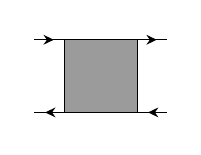
\begin{tikzpicture}[x=0.75pt,y=0.75pt,yscale=-0.7,xscale=0.7, baseline=(XXXX.south) ]
\path (0,68);\path (100,0);\draw    ($(current bounding box.center)+(0,0.3em)$) node [anchor=south] (XXXX) {};
%Straight Lines [id:da22806809134155182] 
\draw    (4.5,8.33) -- (25.33,8.33) ;
%Shape: Square [id:dp6031954177008783] 
\draw  [fill={rgb, 255:red, 155; green, 155; blue, 155 }  ,fill opacity=1 ] (25.33,8.33) -- (75.33,8.33) -- (75.33,58.33) -- (25.33,58.33) -- cycle ;
%Straight Lines [id:da15762936919893056] 
\draw    (14.92,8.33) -- (14.97,8.33) ;
\draw [shift={(17.97,8.33)}, rotate = 180] [fill={rgb, 255:red, 0; green, 0; blue, 0 }  ][line width=0.08]  [draw opacity=0] (7.14,-3.43) -- (0,0) -- (7.14,3.43) -- (4.74,0) -- cycle    ;
%Straight Lines [id:da5710396640221285] 
\draw    (75.33,8.33) -- (96.17,8.33) ;
%Straight Lines [id:da22008735912775146] 
\draw    (85.75,8.33) -- (85.81,8.33) ;
\draw [shift={(88.81,8.33)}, rotate = 180] [fill={rgb, 255:red, 0; green, 0; blue, 0 }  ][line width=0.08]  [draw opacity=0] (7.14,-3.43) -- (0,0) -- (7.14,3.43) -- (4.74,0) -- cycle    ;
%Straight Lines [id:da10139312138178957] 
\draw    (4.5,58.33) -- (25.33,58.33) ;
%Straight Lines [id:da40962399415083883] 
\draw    (14.92,58.33) ;
\draw [shift={(12.04,58.33)}, rotate = 360] [fill={rgb, 255:red, 0; green, 0; blue, 0 }  ][line width=0.08]  [draw opacity=0] (7.14,-3.43) -- (0,0) -- (7.14,3.43) -- (4.74,0) -- cycle    ;
%Straight Lines [id:da7345734656357314] 
\draw    (85.75,58.33) ;
\draw [shift={(82.87,58.33)}, rotate = 360] [fill={rgb, 255:red, 0; green, 0; blue, 0 }  ][line width=0.08]  [draw opacity=0] (7.14,-3.43) -- (0,0) -- (7.14,3.43) -- (4.74,0) -- cycle    ;
%Straight Lines [id:da9940525711272465] 
\draw    (75.33,58.33) -- (96.17,58.33) ;
\end{tikzpicture}
=\tikzset{every picture/.style={line width=0.75pt}} %set default line width to 0.75pt        
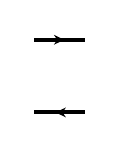
\begin{tikzpicture}[x=0.75pt,y=0.75pt,yscale=-0.7,xscale=0.7, baseline=(XXXX.south) ]
\path (0,68);\path (48.833335876464844,0);\draw    ($(current bounding box.center)+(0,0.3em)$) node [anchor=south] (XXXX) {};
%Straight Lines [id:da5265311146690066] 
\draw [line width=1.5]    (4.5,58.33) -- (39.7,58.33) ;
%Straight Lines [id:da39247742063916924] 
\draw [line width=1.5]    (4.5,8.33) -- (39.7,8.33) ;
%Straight Lines [id:da8442625080101569] 
\draw    (22.1,8.33) -- (22.15,8.33) ;
\draw [shift={(25.15,8.33)}, rotate = 180] [fill={rgb, 255:red, 0; green, 0; blue, 0 }  ][line width=0.08]  [draw opacity=0] (7.14,-3.43) -- (0,0) -- (7.14,3.43) -- (4.74,0) -- cycle    ;
%Straight Lines [id:da3954126655033694] 
\draw    (22.1,58.33) ;
\draw [shift={(19.22,58.33)}, rotate = 360] [fill={rgb, 255:red, 0; green, 0; blue, 0 }  ][line width=0.08]  [draw opacity=0] (7.14,-3.43) -- (0,0) -- (7.14,3.43) -- (4.74,0) -- cycle    ;
\end{tikzpicture}
+\tikzset{every picture/.style={line width=0.75pt}} %set default line width to 0.75pt        
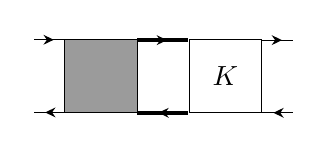
\begin{tikzpicture}[x=0.75pt,y=0.75pt,yscale=-0.7,xscale=0.7, baseline=(XXXX.south) ]
\path (0,68);\path (190.6666717529297,0);\draw    ($(current bounding box.center)+(0,0.3em)$) node [anchor=south] (XXXX) {};
%Straight Lines [id:da7911155113251196] 
\draw    (4.5,8.33) -- (25.33,8.33) ;
%Shape: Square [id:dp19428573744734168] 
\draw  [fill={rgb, 255:red, 155; green, 155; blue, 155 }  ,fill opacity=1 ] (25.33,8.33) -- (75.33,8.33) -- (75.33,58.33) -- (25.33,58.33) -- cycle ;
%Straight Lines [id:da7010679581498145] 
\draw    (14.92,8.33) -- (14.97,8.33) ;
\draw [shift={(17.97,8.33)}, rotate = 180] [fill={rgb, 255:red, 0; green, 0; blue, 0 }  ][line width=0.08]  [draw opacity=0] (7.14,-3.43) -- (0,0) -- (7.14,3.43) -- (4.74,0) -- cycle    ;
%Straight Lines [id:da8907255106568688] 
\draw    (161.58,8.58) -- (182.42,8.58) ;
%Straight Lines [id:da25112705787998446] 
\draw    (172,8.58) -- (172.06,8.58) ;
\draw [shift={(175.06,8.58)}, rotate = 180] [fill={rgb, 255:red, 0; green, 0; blue, 0 }  ][line width=0.08]  [draw opacity=0] (7.14,-3.43) -- (0,0) -- (7.14,3.43) -- (4.74,0) -- cycle    ;
%Straight Lines [id:da15475660740271446] 
\draw    (172,58.58) ;
\draw [shift={(169.12,58.58)}, rotate = 360] [fill={rgb, 255:red, 0; green, 0; blue, 0 }  ][line width=0.08]  [draw opacity=0] (7.14,-3.43) -- (0,0) -- (7.14,3.43) -- (4.74,0) -- cycle    ;
%Straight Lines [id:da5842351849562553] 
\draw    (161.58,58.58) -- (182.42,58.58) ;
%Straight Lines [id:da7087700682172653] 
\draw    (4.5,58.33) -- (25.33,58.33) ;
%Straight Lines [id:da49703420824140654] 
\draw    (14.92,58.33) ;
\draw [shift={(12.04,58.33)}, rotate = 360] [fill={rgb, 255:red, 0; green, 0; blue, 0 }  ][line width=0.08]  [draw opacity=0] (7.14,-3.43) -- (0,0) -- (7.14,3.43) -- (4.74,0) -- cycle    ;
%Straight Lines [id:da5594862502970488] 
\draw [line width=1.5]    (75.25,58.58) -- (110.45,58.58) ;
%Straight Lines [id:da7706538069595303] 
\draw [line width=1.5]    (75.25,8.58) -- (110.45,8.58) ;
%Straight Lines [id:da49897124888842126] 
\draw    (92.85,8.58) -- (92.9,8.58) ;
\draw [shift={(95.9,8.58)}, rotate = 180] [fill={rgb, 255:red, 0; green, 0; blue, 0 }  ][line width=0.08]  [draw opacity=0] (7.14,-3.43) -- (0,0) -- (7.14,3.43) -- (4.74,0) -- cycle    ;
%Straight Lines [id:da896337553631787] 
\draw    (92.85,58.58) ;
\draw [shift={(89.97,58.58)}, rotate = 360] [fill={rgb, 255:red, 0; green, 0; blue, 0 }  ][line width=0.08]  [draw opacity=0] (7.14,-3.43) -- (0,0) -- (7.14,3.43) -- (4.74,0) -- cycle    ;
%Shape: Square [id:dp2523741527250978] 
\draw  [fill={rgb, 255:red, 255; green, 255; blue, 255 }  ,fill opacity=1 ] (111.08,8.33) -- (161.08,8.33) -- (161.08,58.33) -- (111.08,58.33) -- cycle ;
% Text Node
\draw (136.08,33.33) node    {$K$};
\end{tikzpicture}
    \end{equation}
    
    \vspace{0.5cm}

    \textbf{What we need} Linear response of single-electron under external field = BSE 
    (simplest single-electron theory: QBE)
    \vspace{-0.1cm}
    \begin{equation}
        \protect\tikzset{every picture/.style={line width=0.75pt}} %set default line width to 0.75pt        
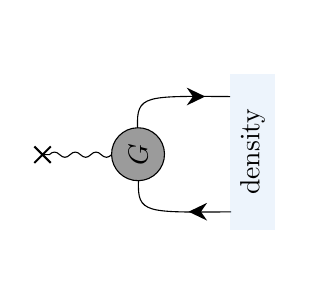
\begin{tikzpicture}[x=0.75pt,y=0.75pt,yscale=-1,xscale=1, baseline=(XXXX.south) ]
\path (0,115);\path (127.33334350585938,0);\draw    ($(current bounding box.center)+(0,0.3em)$) node [anchor=south] (XXXX) {};
%Shape: Circle [id:dp8418847107385614] 
\draw  [fill={rgb, 255:red, 155; green, 155; blue, 155 }  ,fill opacity=1 ] (53.4,73.72) .. controls (46.35,73.84) and (40.55,68.23) .. (40.43,61.19) .. controls (40.31,54.15) and (45.91,48.34) .. (52.95,48.22) .. controls (60,48.1) and (65.8,53.71) .. (65.92,60.75) .. controls (66.04,67.79) and (60.44,73.59) .. (53.4,73.72) -- cycle ;
%Straight Lines [id:da27727362427127455] 
\draw    (40.43,61.19) .. controls (38.76,62.86) and (37.1,62.86) .. (35.43,61.19) .. controls (33.76,59.52) and (32.1,59.52) .. (30.43,61.19) .. controls (28.76,62.86) and (27.1,62.86) .. (25.43,61.19) .. controls (23.76,59.52) and (22.1,59.52) .. (20.43,61.19) .. controls (18.76,62.86) and (17.1,62.86) .. (15.43,61.19) .. controls (13.76,59.52) and (12.1,59.52) .. (10.43,61.19) -- (7.17,61.19) -- (7.17,61.19) ;
\draw [shift={(7.17,61.19)}, rotate = 225] [color={rgb, 255:red, 0; green, 0; blue, 0 }  ][line width=0.75]    (-5.59,0) -- (5.59,0)(0,5.59) -- (0,-5.59)   ;
%Curve Lines [id:da35151936874808354] 
\draw    (52.95,48.22) .. controls (52.29,32.21) and (56.54,32.96) .. (97.54,33.19) ;
%Curve Lines [id:da556586976499901] 
\draw    (53.4,73.72) .. controls (52.73,89.72) and (56.98,88.97) .. (97.98,88.75) ;
%Straight Lines [id:da11356715352037416] 
\draw    (75.04,33.17) -- (82.54,33.17) ;
\draw [shift={(85.54,33.17)}, rotate = 180] [fill={rgb, 255:red, 0; green, 0; blue, 0 }  ][line width=0.08]  [draw opacity=0] (8.93,-4.29) -- (0,0) -- (8.93,4.29) -- (5.93,0) -- cycle    ;
%Straight Lines [id:da5122608194893252] 
\draw    (81.04,88.67) -- (80.54,88.67) ;
\draw [shift={(77.54,88.67)}, rotate = 360] [fill={rgb, 255:red, 0; green, 0; blue, 0 }  ][line width=0.08]  [draw opacity=0] (8.93,-4.29) -- (0,0) -- (8.93,4.29) -- (5.93,0) -- cycle    ;
%Shape: Rectangle [id:dp5571429910759773] 
\draw  [draw opacity=0][fill={rgb, 255:red, 74; green, 144; blue, 226 }  ,fill opacity=0.1 ] (97.54,22.19) -- (119.04,22.19) -- (119.04,97.44) -- (97.54,97.44) -- cycle ;
% Text Node
\draw (53.18,60.97) node  [rotate=-270] [align=left] {$\displaystyle G$};
% Text Node
\draw (108.29,59.81) node  [rotate=-270] [align=left] {density};
\end{tikzpicture}
=\tikzset{every picture/.style={line width=0.75pt}} %set default line width to 0.75pt        
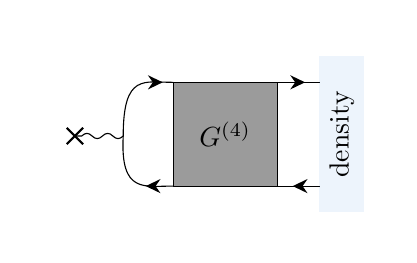
\begin{tikzpicture}[x=0.75pt,y=0.75pt,yscale=-1,xscale=1, baseline=(XXXX.south) ]
\path (0,100);\path (174,0);\draw    ($(current bounding box.center)+(0,0.3em)$) node [anchor=south] (XXXX) {};
%Shape: Square [id:dp18428995702891116] 
\draw  [fill={rgb, 255:red, 155; green, 155; blue, 155 }  ,fill opacity=1 ] (70.17,26.33) -- (120.17,26.33) -- (120.17,76.33) -- (70.17,76.33) -- cycle ;
%Straight Lines [id:da9168863590107177] 
\draw    (62,26.33) -- (62.06,26.33) ;
\draw [shift={(65.06,26.33)}, rotate = 180] [fill={rgb, 255:red, 0; green, 0; blue, 0 }  ][line width=0.08]  [draw opacity=0] (7.14,-3.43) -- (0,0) -- (7.14,3.43) -- (4.74,0) -- cycle    ;
%Straight Lines [id:da9974081789895775] 
\draw    (120.17,26.33) -- (141,26.33) ;
%Straight Lines [id:da9844170706019146] 
\draw    (130.58,26.33) -- (130.64,26.33) ;
\draw [shift={(133.64,26.33)}, rotate = 180] [fill={rgb, 255:red, 0; green, 0; blue, 0 }  ][line width=0.08]  [draw opacity=0] (7.14,-3.43) -- (0,0) -- (7.14,3.43) -- (4.74,0) -- cycle    ;
%Straight Lines [id:da35484421445884906] 
\draw    (59.75,76.33) ;
\draw [shift={(56.88,76.33)}, rotate = 360] [fill={rgb, 255:red, 0; green, 0; blue, 0 }  ][line width=0.08]  [draw opacity=0] (7.14,-3.43) -- (0,0) -- (7.14,3.43) -- (4.74,0) -- cycle    ;
%Straight Lines [id:da7829107592696085] 
\draw    (130.58,76.33) ;
\draw [shift={(127.71,76.33)}, rotate = 360] [fill={rgb, 255:red, 0; green, 0; blue, 0 }  ][line width=0.08]  [draw opacity=0] (7.14,-3.43) -- (0,0) -- (7.14,3.43) -- (4.74,0) -- cycle    ;
%Straight Lines [id:da7163534152969595] 
\draw    (120.17,76.33) -- (141,76.33) ;
%Shape: Rectangle [id:dp6933567821360969] 
\draw  [draw opacity=0][fill={rgb, 255:red, 74; green, 144; blue, 226 }  ,fill opacity=0.1 ] (140.58,13.75) -- (162.08,13.75) -- (162.08,89) -- (140.58,89) -- cycle ;
%Curve Lines [id:da8015668095588748] 
\draw    (46.03,52.19) .. controls (46.03,21.69) and (56.28,26.44) .. (70.17,26.33) ;
%Curve Lines [id:da6612866448888022] 
\draw    (46.03,52.19) .. controls (44.53,80.19) and (56.28,76.23) .. (70.17,76.33) ;
%Straight Lines [id:da6953811427117405] 
\draw    (46.03,52.19) .. controls (44.36,53.86) and (42.7,53.86) .. (41.03,52.19) .. controls (39.36,50.52) and (37.7,50.52) .. (36.03,52.19) .. controls (34.36,53.86) and (32.7,53.86) .. (31.03,52.19) .. controls (29.36,50.52) and (27.7,50.52) .. (26.03,52.19) -- (22.78,52.19) -- (22.78,52.19) ;
\draw [shift={(22.78,52.19)}, rotate = 225] [color={rgb, 255:red, 0; green, 0; blue, 0 }  ][line width=0.75]    (-5.59,0) -- (5.59,0)(0,5.59) -- (0,-5.59)   ;
% Text Node
\draw (151.33,51.38) node  [rotate=-270] [align=left] {density};
% Text Node
\draw (95.17,51.33) node    {$G^{( 4)}$};
\end{tikzpicture}
    \end{equation} 
    
    \textbf{Next step: relation between $K$ and $\Sigma$}
\end{frame}

\begin{frame}
    \frametitle{Linking $\Sigma$ with $K$}

    \textbf{Linear response of a single self-energy diagram}
    
    
    \begin{equation}
        \protect\Sigma =\tikzset{every picture/.style={line width=0.75pt}} %set default line width to 0.75pt        
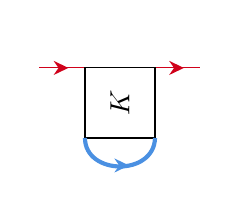
\begin{tikzpicture}[x=0.75pt,y=0.75pt,yscale=-1,xscale=1, baseline=(XXXX.south) ]
\path (0,77);\path (89.33333587646484,0);\draw    ($(current bounding box.center)+(0,0.3em)$) node [anchor=south] (XXXX) {};
%Straight Lines [id:da8382131249777933] 
\draw [color={rgb, 255:red, 208; green, 2; blue, 27 }  ,draw opacity=1 ]   (5.5,19.39) -- (27.61,19.39) ;
%Straight Lines [id:da7240261607790925] 
\draw [color={rgb, 255:red, 208; green, 2; blue, 27 }  ,draw opacity=1 ]   (61.36,19.39) -- (83.06,19.39) ;
%Straight Lines [id:da1930777146623066] 
\draw [color={rgb, 255:red, 208; green, 2; blue, 27 }  ,draw opacity=1 ]   (16.56,19.39) -- (16.61,19.39) ;
\draw [shift={(19.61,19.39)}, rotate = 180] [fill={rgb, 255:red, 208; green, 2; blue, 27 }  ,fill opacity=1 ][line width=0.08]  [draw opacity=0] (7.14,-3.43) -- (0,0) -- (7.14,3.43) -- (4.74,0) -- cycle    ;
%Straight Lines [id:da07919795645711414] 
\draw [color={rgb, 255:red, 208; green, 2; blue, 27 }  ,draw opacity=1 ]   (72.21,19.39) -- (72.27,19.39) ;
\draw [shift={(75.27,19.39)}, rotate = 180] [fill={rgb, 255:red, 208; green, 2; blue, 27 }  ,fill opacity=1 ][line width=0.08]  [draw opacity=0] (7.14,-3.43) -- (0,0) -- (7.14,3.43) -- (4.74,0) -- cycle    ;
%Shape: Square [id:dp5873383974217354] 
\draw   (27.61,19.39) -- (61.36,19.39) -- (61.36,53.14) -- (27.61,53.14) -- cycle ;
%Curve Lines [id:da4568403322032253] 
\draw [color={rgb, 255:red, 74; green, 144; blue, 226 }  ,draw opacity=1 ][line width=1.5]    (27.61,53.14) .. controls (27.61,71.19) and (60.86,71.69) .. (61.36,53.14) ;
%Straight Lines [id:da7186505275056507] 
\draw [color={rgb, 255:red, 74; green, 144; blue, 226 }  ,draw opacity=1 ]   (45.81,66.39) -- (45.86,66.39) ;
\draw [shift={(48.86,66.39)}, rotate = 180] [fill={rgb, 255:red, 74; green, 144; blue, 226 }  ,fill opacity=1 ][line width=0.08]  [draw opacity=0] (7.14,-3.43) -- (0,0) -- (7.14,3.43) -- (4.74,0) -- cycle    ;
% Text Node
\draw (44.49,36.26) node  [rotate=-270]  {$K$};
\end{tikzpicture}
\stackrel{\text{driving}}{\longrightarrow }\tikzset{every picture/.style={line width=0.75pt}} %set default line width to 0.75pt        
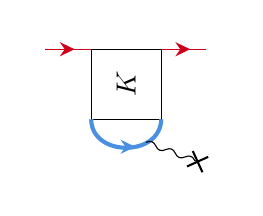
\begin{tikzpicture}[x=0.75pt,y=0.75pt,yscale=-1,xscale=1, baseline=(XXXX.south) ]
\path (0,77);\path (100,0);\draw    ($(current bounding box.center)+(0,0.3em)$) node [anchor=south] (XXXX) {};
%Straight Lines [id:da7828028568002114] 
\draw [color={rgb, 255:red, 208; green, 2; blue, 27 }  ,draw opacity=1 ]   (8.5,10.39) -- (30.61,10.39) ;
%Straight Lines [id:da5090451707270729] 
\draw [color={rgb, 255:red, 208; green, 2; blue, 27 }  ,draw opacity=1 ]   (64.36,10.39) -- (86.06,10.39) ;
%Straight Lines [id:da54602000208046] 
\draw [color={rgb, 255:red, 208; green, 2; blue, 27 }  ,draw opacity=1 ]   (19.56,10.39) -- (19.61,10.39) ;
\draw [shift={(22.61,10.39)}, rotate = 180] [fill={rgb, 255:red, 208; green, 2; blue, 27 }  ,fill opacity=1 ][line width=0.08]  [draw opacity=0] (7.14,-3.43) -- (0,0) -- (7.14,3.43) -- (4.74,0) -- cycle    ;
%Straight Lines [id:da23332419347589273] 
\draw [color={rgb, 255:red, 208; green, 2; blue, 27 }  ,draw opacity=1 ]   (75.21,10.39) -- (75.27,10.39) ;
\draw [shift={(78.27,10.39)}, rotate = 180] [fill={rgb, 255:red, 208; green, 2; blue, 27 }  ,fill opacity=1 ][line width=0.08]  [draw opacity=0] (7.14,-3.43) -- (0,0) -- (7.14,3.43) -- (4.74,0) -- cycle    ;
%Shape: Square [id:dp039216724440099604] 
\draw   (30.61,10.39) -- (64.36,10.39) -- (64.36,44.14) -- (30.61,44.14) -- cycle ;
%Curve Lines [id:da5231570845294202] 
\draw [color={rgb, 255:red, 74; green, 144; blue, 226 }  ,draw opacity=1 ][line width=1.5]    (30.61,44.14) .. controls (30.61,62.19) and (63.86,62.69) .. (64.36,44.14) ;
%Straight Lines [id:da2778689604122657] 
\draw [color={rgb, 255:red, 74; green, 144; blue, 226 }  ,draw opacity=1 ]   (48.81,57.39) -- (48.86,57.39) ;
\draw [shift={(51.86,57.39)}, rotate = 180] [fill={rgb, 255:red, 74; green, 144; blue, 226 }  ,fill opacity=1 ][line width=0.08]  [draw opacity=0] (7.14,-3.43) -- (0,0) -- (7.14,3.43) -- (4.74,0) -- cycle    ;
%Straight Lines [id:da35619683062191276] 
\draw    (57.08,55.25) .. controls (59.23,54.28) and (60.79,54.86) .. (61.76,57.01) .. controls (62.74,59.16) and (64.3,59.74) .. (66.45,58.76) .. controls (68.6,57.79) and (70.16,58.37) .. (71.13,60.52) .. controls (72.1,62.67) and (73.66,63.25) .. (75.81,62.28) .. controls (77.96,61.3) and (79.52,61.88) .. (80.49,64.03) -- (81.88,64.55) -- (81.88,64.55) ;
\draw [shift={(81.88,64.55)}, rotate = 65.57] [color={rgb, 255:red, 0; green, 0; blue, 0 }  ][line width=0.75]    (-5.59,0) -- (5.59,0)(0,5.59) -- (0,-5.59)   ;
% Text Node
\draw (47.49,27.26) node  [rotate=-270]  {$K$};
\end{tikzpicture}
\stackrel{\text{linear res.}}{\longrightarrow }\tikzset{every picture/.style={line width=0.75pt}} %set default line width to 0.75pt        
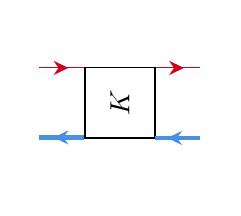
\begin{tikzpicture}[x=0.75pt,y=0.75pt,yscale=-1,xscale=1, baseline=(XXXX.south) ]
\path (0,77);\path (89.33333587646484,0);\draw    ($(current bounding box.center)+(0,0.3em)$) node [anchor=south] (XXXX) {};
%Straight Lines [id:da7115676979609427] 
\draw [color={rgb, 255:red, 208; green, 2; blue, 27 }  ,draw opacity=1 ]   (5.5,19.39) -- (27.61,19.39) ;
%Straight Lines [id:da8226174984587384] 
\draw [color={rgb, 255:red, 208; green, 2; blue, 27 }  ,draw opacity=1 ]   (61.36,19.39) -- (83.06,19.39) ;
%Straight Lines [id:da25326861646368304] 
\draw [color={rgb, 255:red, 208; green, 2; blue, 27 }  ,draw opacity=1 ]   (16.56,19.39) -- (16.61,19.39) ;
\draw [shift={(19.61,19.39)}, rotate = 180] [fill={rgb, 255:red, 208; green, 2; blue, 27 }  ,fill opacity=1 ][line width=0.08]  [draw opacity=0] (7.14,-3.43) -- (0,0) -- (7.14,3.43) -- (4.74,0) -- cycle    ;
%Straight Lines [id:da34362814096939687] 
\draw [color={rgb, 255:red, 208; green, 2; blue, 27 }  ,draw opacity=1 ]   (72.21,19.39) -- (72.27,19.39) ;
\draw [shift={(75.27,19.39)}, rotate = 180] [fill={rgb, 255:red, 208; green, 2; blue, 27 }  ,fill opacity=1 ][line width=0.08]  [draw opacity=0] (7.14,-3.43) -- (0,0) -- (7.14,3.43) -- (4.74,0) -- cycle    ;
%Shape: Square [id:dp2058159278792857] 
\draw   (27.61,19.39) -- (61.36,19.39) -- (61.36,53.14) -- (27.61,53.14) -- cycle ;
%Straight Lines [id:da7878855943317369] 
\draw [color={rgb, 255:red, 74; green, 144; blue, 226 }  ,draw opacity=1 ][line width=1.5]    (61.36,53.14) -- (83.06,53.14) ;
%Straight Lines [id:da23573675788589998] 
\draw [color={rgb, 255:red, 74; green, 144; blue, 226 }  ,draw opacity=1 ]   (72.21,53.14) -- (70.27,53.14) ;
\draw [shift={(67.27,53.14)}, rotate = 360] [fill={rgb, 255:red, 74; green, 144; blue, 226 }  ,fill opacity=1 ][line width=0.08]  [draw opacity=0] (7.14,-3.43) -- (0,0) -- (7.14,3.43) -- (4.74,0) -- cycle    ;
%Straight Lines [id:da18492619986102254] 
\draw [color={rgb, 255:red, 74; green, 144; blue, 226 }  ,draw opacity=1 ][line width=1.5]    (5.64,52.89) -- (27.33,52.89) ;
%Straight Lines [id:da9508478089699361] 
\draw [color={rgb, 255:red, 74; green, 144; blue, 226 }  ,draw opacity=1 ]   (13.48,52.89) ;
\draw [shift={(12.54,52.89)}, rotate = 360] [fill={rgb, 255:red, 74; green, 144; blue, 226 }  ,fill opacity=1 ][line width=0.08]  [draw opacity=0] (7.14,-3.43) -- (0,0) -- (7.14,3.43) -- (4.74,0) -- cycle    ;
% Text Node
\draw (44.49,36.26) node  [rotate=-270]  {$K$};
\end{tikzpicture}
    \end{equation}


\end{frame}

\begin{frame}
    \frametitle{Linking $\Sigma$ with $K$}

    \textbf{Whole picture} 
    
    \begin{equation}
        \protect\begin{array}{{>{\displaystyle}l}}
    \tikzset{every picture/.style={line width=0.75pt}} %set default line width to 0.75pt        
    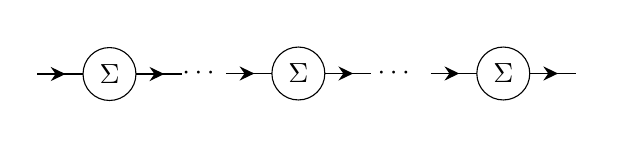
\begin{tikzpicture}[x=0.75pt,y=0.75pt,yscale=-1,xscale=1, baseline=(XXXX.south) ]
    \path (0,48);\path (272,0);\draw    ($(current bounding box.center)+(0,0.3em)$) node [anchor=south] (XXXX) {};
    %Straight Lines [id:da7730421935461638] 
    \draw    (95.55,22.08) -- (117.67,22.08) ;
    \draw [shift={(109.21,22.08)}, rotate = 180] [fill={rgb, 255:red, 0; green, 0; blue, 0 }  ][line width=0.08]  [draw opacity=0] (7.14,-3.43) -- (0,0) -- (7.14,3.43) -- (4.74,0) -- cycle    ;
    %Straight Lines [id:da15424393729989738] 
    \draw    (143.17,22.08) -- (165.28,22.08) ;
    \draw [shift={(156.82,22.08)}, rotate = 180] [fill={rgb, 255:red, 0; green, 0; blue, 0 }  ][line width=0.08]  [draw opacity=0] (7.14,-3.43) -- (0,0) -- (7.14,3.43) -- (4.74,0) -- cycle    ;
    %Shape: Circle [id:dp8494816441450308] 
    \draw   (117.67,22.08) .. controls (117.67,15.04) and (123.38,9.33) .. (130.42,9.33) .. controls (137.46,9.33) and (143.17,15.04) .. (143.17,22.08) .. controls (143.17,29.12) and (137.46,34.83) .. (130.42,34.83) .. controls (123.38,34.83) and (117.67,29.12) .. (117.67,22.08) -- cycle ;
    %Straight Lines [id:da7003617558961506] 
    \draw    (194.28,22.08) -- (216.4,22.08) ;
    \draw [shift={(207.94,22.08)}, rotate = 180] [fill={rgb, 255:red, 0; green, 0; blue, 0 }  ][line width=0.08]  [draw opacity=0] (7.14,-3.43) -- (0,0) -- (7.14,3.43) -- (4.74,0) -- cycle    ;
    %Shape: Circle [id:dp13551607571889623] 
    \draw   (216.4,22.08) .. controls (216.4,15.04) and (222.1,9.33) .. (229.15,9.33) .. controls (236.19,9.33) and (241.9,15.04) .. (241.9,22.08) .. controls (241.9,29.12) and (236.19,34.83) .. (229.15,34.83) .. controls (222.1,34.83) and (216.4,29.12) .. (216.4,22.08) -- cycle ;
    %Straight Lines [id:da2754236095535514] 
    \draw    (241.9,22.08) -- (264.01,22.08) ;
    \draw [shift={(255.55,22.08)}, rotate = 180] [fill={rgb, 255:red, 0; green, 0; blue, 0 }  ][line width=0.08]  [draw opacity=0] (7.14,-3.43) -- (0,0) -- (7.14,3.43) -- (4.74,0) -- cycle    ;
    %Straight Lines [id:da3425218625555646] 
    \draw    (4.55,22.33) -- (26.67,22.33) ;
    \draw [shift={(18.21,22.33)}, rotate = 180] [fill={rgb, 255:red, 0; green, 0; blue, 0 }  ][line width=0.08]  [draw opacity=0] (7.14,-3.43) -- (0,0) -- (7.14,3.43) -- (4.74,0) -- cycle    ;
    %Straight Lines [id:da9579670889213272] 
    \draw    (52.17,22.33) -- (74.28,22.33) ;
    \draw [shift={(65.82,22.33)}, rotate = 180] [fill={rgb, 255:red, 0; green, 0; blue, 0 }  ][line width=0.08]  [draw opacity=0] (7.14,-3.43) -- (0,0) -- (7.14,3.43) -- (4.74,0) -- cycle    ;
    %Shape: Circle [id:dp9811386287790373] 
    \draw   (26.67,22.33) .. controls (26.67,15.29) and (32.38,9.58) .. (39.42,9.58) .. controls (46.46,9.58) and (52.17,15.29) .. (52.17,22.33) .. controls (52.17,29.37) and (46.46,35.08) .. (39.42,35.08) .. controls (32.38,35.08) and (26.67,29.37) .. (26.67,22.33) -- cycle ;
    % Text Node
    \draw (130.42,22.08) node   [align=left] {$\displaystyle \Sigma $};
    % Text Node
    \draw (167.28,22.08) node [anchor=west] [inner sep=0.75pt]   [align=left] {$\displaystyle \cdots $};
    % Text Node
    \draw (93.55,22.08) node [anchor=east] [inner sep=0.75pt]   [align=left] {$\displaystyle \cdots $};
    % Text Node
    \draw (229.15,22.08) node   [align=left] {$\displaystyle \Sigma $};
    % Text Node
    \draw (39.42,22.33) node   [align=left] {$\displaystyle \Sigma $};
    \end{tikzpicture}
    \\
    \stackrel{\text{linear res.}}{\longrightarrow }\tikzset{every picture/.style={line width=0.75pt}} %set default line width to 0.75pt        
    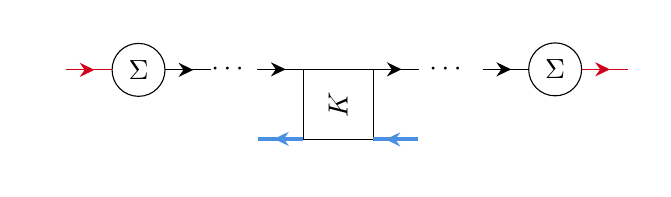
\begin{tikzpicture}[x=0.75pt,y=0.75pt,yscale=-1,xscale=1, baseline=(XXXX.south) ]
    \path (0,68);\path (296.3333435058594,0);\draw    ($(current bounding box.center)+(0,0.3em)$) node [anchor=south] (XXXX) {};
    %Straight Lines [id:da7765799409174068] 
    \draw    (166.5,20.08) -- (188.61,20.08) ;
    \draw [shift={(180.16,20.08)}, rotate = 180] [fill={rgb, 255:red, 0; green, 0; blue, 0 }  ][line width=0.08]  [draw opacity=0] (7.14,-3.43) -- (0,0) -- (7.14,3.43) -- (4.74,0) -- cycle    ;
    %Straight Lines [id:da6304991238150759] 
    \draw    (219.27,20.08) -- (241.39,20.08) ;
    \draw [shift={(232.93,20.08)}, rotate = 180] [fill={rgb, 255:red, 0; green, 0; blue, 0 }  ][line width=0.08]  [draw opacity=0] (7.14,-3.43) -- (0,0) -- (7.14,3.43) -- (4.74,0) -- cycle    ;
    %Shape: Circle [id:dp5767170987507564] 
    \draw   (241.39,20.08) .. controls (241.39,13.04) and (247.09,7.33) .. (254.14,7.33) .. controls (261.18,7.33) and (266.89,13.04) .. (266.89,20.08) .. controls (266.89,27.12) and (261.18,32.83) .. (254.14,32.83) .. controls (247.09,32.83) and (241.39,27.12) .. (241.39,20.08) -- cycle ;
    %Straight Lines [id:da9757455340617616] 
    \draw [color={rgb, 255:red, 208; green, 2; blue, 27 }  ,draw opacity=1 ]   (266.89,20.08) -- (289,20.08) ;
    \draw [shift={(280.54,20.08)}, rotate = 180] [fill={rgb, 255:red, 208; green, 2; blue, 27 }  ,fill opacity=1 ][line width=0.08]  [draw opacity=0] (7.14,-3.43) -- (0,0) -- (7.14,3.43) -- (4.74,0) -- cycle    ;
    %Straight Lines [id:da17687860465606242] 
    \draw [color={rgb, 255:red, 208; green, 2; blue, 27 }  ,draw opacity=1 ]   (18.54,20.33) -- (40.66,20.33) ;
    \draw [shift={(32.2,20.33)}, rotate = 180] [fill={rgb, 255:red, 208; green, 2; blue, 27 }  ,fill opacity=1 ][line width=0.08]  [draw opacity=0] (7.14,-3.43) -- (0,0) -- (7.14,3.43) -- (4.74,0) -- cycle    ;
    %Straight Lines [id:da9551463276321575] 
    \draw    (66.16,20.33) -- (88.27,20.33) ;
    \draw [shift={(79.81,20.33)}, rotate = 180] [fill={rgb, 255:red, 0; green, 0; blue, 0 }  ][line width=0.08]  [draw opacity=0] (7.14,-3.43) -- (0,0) -- (7.14,3.43) -- (4.74,0) -- cycle    ;
    %Shape: Circle [id:dp18022024253349378] 
    \draw   (40.66,20.33) .. controls (40.66,13.29) and (46.36,7.58) .. (53.41,7.58) .. controls (60.45,7.58) and (66.16,13.29) .. (66.16,20.33) .. controls (66.16,27.37) and (60.45,33.08) .. (53.41,33.08) .. controls (46.36,33.08) and (40.66,27.37) .. (40.66,20.33) -- cycle ;
    %Shape: Square [id:dp173511178718035] 
    \draw   (132.75,20.08) -- (166.5,20.08) -- (166.5,53.83) -- (132.75,53.83) -- cycle ;
    %Straight Lines [id:da4478490058833322] 
    \draw    (110.64,20.08) -- (132.75,20.08) ;
    \draw [shift={(124.29,20.08)}, rotate = 180] [fill={rgb, 255:red, 0; green, 0; blue, 0 }  ][line width=0.08]  [draw opacity=0] (7.14,-3.43) -- (0,0) -- (7.14,3.43) -- (4.74,0) -- cycle    ;
    %Straight Lines [id:da9602850908691027] 
    \draw [color={rgb, 255:red, 74; green, 144; blue, 226 }  ,draw opacity=1 ][line width=1.5]    (111.05,53.83) -- (132.75,53.83) ;
    %Straight Lines [id:da991838493690111] 
    \draw [color={rgb, 255:red, 74; green, 144; blue, 226 }  ,draw opacity=1 ]   (119.65,53.58) ;
    \draw [shift={(118.71,53.58)}, rotate = 360] [fill={rgb, 255:red, 74; green, 144; blue, 226 }  ,fill opacity=1 ][line width=0.08]  [draw opacity=0] (7.14,-3.43) -- (0,0) -- (7.14,3.43) -- (4.74,0) -- cycle    ;
    %Straight Lines [id:da7138945428047838] 
    \draw [color={rgb, 255:red, 74; green, 144; blue, 226 }  ,draw opacity=1 ][line width=1.5]    (166.5,53.83) -- (188.2,53.83) ;
    %Straight Lines [id:da44161029156064124] 
    \draw [color={rgb, 255:red, 74; green, 144; blue, 226 }  ,draw opacity=1 ]   (177.35,53.83) -- (175.4,53.83) ;
    \draw [shift={(172.4,53.83)}, rotate = 360] [fill={rgb, 255:red, 74; green, 144; blue, 226 }  ,fill opacity=1 ][line width=0.08]  [draw opacity=0] (7.14,-3.43) -- (0,0) -- (7.14,3.43) -- (4.74,0) -- cycle    ;
    % Text Node
    \draw (192.27,20.08) node [anchor=west] [inner sep=0.75pt]   [align=left] {$\displaystyle \cdots $};
    % Text Node
    \draw (107.54,20.08) node [anchor=east] [inner sep=0.75pt]   [align=left] {$\displaystyle \cdots $};
    % Text Node
    \draw (254.14,20.08) node   [align=left] {$\displaystyle \Sigma $};
    % Text Node
    \draw (53.41,20.33) node   [align=left] {$\displaystyle \Sigma $};
    % Text Node
    \draw (149.63,36.96) node  [rotate=-270]  {$K$};
    \end{tikzpicture}
    \\
    =\tikzset{every picture/.style={line width=0.75pt}} %set default line width to 0.75pt        
    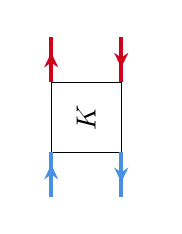
\begin{tikzpicture}[x=0.75pt,y=0.75pt,yscale=-1,xscale=1, baseline=(XXXX.south) ]
    \path (0,86);\path (61,0);\draw    ($(current bounding box.center)+(0,0.3em)$) node [anchor=south] (XXXX) {};
    %Shape: Square [id:dp044155492377603967] 
    \draw   (45.08,26.33) -- (45.08,60.08) -- (11.33,60.08) -- (11.33,26.33) -- cycle ;
    %Straight Lines [id:da978251106936799] 
    \draw [color={rgb, 255:red, 208; green, 2; blue, 27 }  ,draw opacity=1 ][line width=1.5]    (11.33,4.64) -- (11.33,26.33) ;
    %Straight Lines [id:da36221246059843093] 
    \draw [color={rgb, 255:red, 208; green, 2; blue, 27 }  ,draw opacity=1 ]   (11.33,12.98) ;
    \draw [shift={(11.33,12.04)}, rotate = 90] [fill={rgb, 255:red, 208; green, 2; blue, 27 }  ,fill opacity=1 ][line width=0.08]  [draw opacity=0] (7.14,-3.43) -- (0,0) -- (7.14,3.43) -- (4.74,0) -- cycle    ;
    %Straight Lines [id:da3818367454641727] 
    \draw [color={rgb, 255:red, 74; green, 144; blue, 226 }  ,draw opacity=1 ][line width=1.5]    (11.33,60.08) -- (11.33,81.78) ;
    %Straight Lines [id:da42917124212508795] 
    \draw [color={rgb, 255:red, 74; green, 144; blue, 226 }  ,draw opacity=1 ]   (11.33,70.93) -- (11.33,68.99) ;
    \draw [shift={(11.33,65.99)}, rotate = 90] [fill={rgb, 255:red, 74; green, 144; blue, 226 }  ,fill opacity=1 ][line width=0.08]  [draw opacity=0] (7.14,-3.43) -- (0,0) -- (7.14,3.43) -- (4.74,0) -- cycle    ;
    %Straight Lines [id:da5676567389068676] 
    \draw [color={rgb, 255:red, 208; green, 2; blue, 27 }  ,draw opacity=1 ][line width=1.5]    (45.08,4.64) -- (45.08,26.33) ;
    %Straight Lines [id:da5426804686695461] 
    \draw [color={rgb, 255:red, 208; green, 2; blue, 27 }  ,draw opacity=1 ]   (45.08,22.18) -- (45.08,18.23) ;
    \draw [shift={(45.08,19.23)}, rotate = 270] [fill={rgb, 255:red, 208; green, 2; blue, 27 }  ,fill opacity=1 ][line width=0.08]  [draw opacity=0] (7.14,-3.43) -- (0,0) -- (7.14,3.43) -- (4.74,0) -- cycle    ;
    %Straight Lines [id:da004906008388375849] 
    \draw [color={rgb, 255:red, 74; green, 144; blue, 226 }  ,draw opacity=1 ][line width=1.5]    (45.08,59.89) -- (45.08,81.58) ;
    %Straight Lines [id:da11120487956269187] 
    \draw [color={rgb, 255:red, 74; green, 144; blue, 226 }  ,draw opacity=1 ]   (45.08,77.43) -- (45.08,73.48) ;
    \draw [shift={(45.08,74.48)}, rotate = 270] [fill={rgb, 255:red, 74; green, 144; blue, 226 }  ,fill opacity=1 ][line width=0.08]  [draw opacity=0] (7.14,-3.43) -- (0,0) -- (7.14,3.43) -- (4.74,0) -- cycle    ;
    % Text Node
    \draw (28.21,43.21) node  [rotate=-270]  {$K$};
    \end{tikzpicture}
    \end{array}
    \end{equation}

\end{frame}

\begin{frame}
    \frametitle{Linking $\Sigma$ with $K$}

    \textbf{Example: linear response from time-dependent $GW$ = BSE}
    
    \begin{equation}
        \begin{array}{{>{\displaystyle}l}}
    \Sigma =\tikzset{every picture/.style={line width=0.75pt}} %set default line width to 0.75pt        
    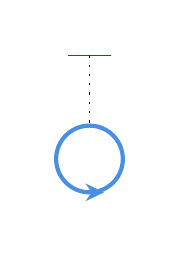
\begin{tikzpicture}[x=0.75pt,y=0.75pt,yscale=-1,xscale=1, baseline=(XXXX.south) ]
    \path (0,95);\path (58.66667175292969,0);\draw    ($(current bounding box.center)+(0,0.3em)$) node [anchor=south] (XXXX) {};
    %Straight Lines [id:da4998816518046578] 
    \draw [color={rgb, 255:red, 208; green, 2; blue, 27 }  ,draw opacity=1 ]   (19.33,13.33) -- (29.78,13.33) ;
    %Straight Lines [id:da4915326171607255] 
    \draw [color={rgb, 255:red, 208; green, 2; blue, 27 }  ,draw opacity=1 ]   (29.78,13.33) -- (40.23,13.33) ;
    %Straight Lines [id:da5880455681975667] 
    \draw  [dash pattern={on 0.84pt off 2.51pt}]  (29.78,13.33) -- (29.78,47.19) ;
    %Shape: Circle [id:dp11061037689839615] 
    \draw  [color={rgb, 255:red, 74; green, 144; blue, 226 }  ,draw opacity=1 ][line width=1.5]  (13.71,63.26) .. controls (13.71,54.38) and (20.9,47.19) .. (29.78,47.19) .. controls (38.66,47.19) and (45.85,54.38) .. (45.85,63.26) .. controls (45.85,72.14) and (38.66,79.33) .. (29.78,79.33) .. controls (20.9,79.33) and (13.71,72.14) .. (13.71,63.26) -- cycle ;
    %Straight Lines [id:da6438867610231551] 
    \draw [color={rgb, 255:red, 74; green, 144; blue, 226 }  ,draw opacity=1 ]   (29.78,79.33) -- (33.78,79.33) ;
    \draw [shift={(36.78,79.33)}, rotate = 180] [fill={rgb, 255:red, 74; green, 144; blue, 226 }  ,fill opacity=1 ][line width=0.08]  [draw opacity=0] (8.93,-4.29) -- (0,0) -- (8.93,4.29) -- (5.93,0) -- cycle    ;
    \end{tikzpicture}
    +\tikzset{every picture/.style={line width=0.75pt}} %set default line width to 0.75pt        
    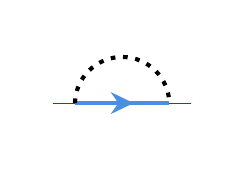
\begin{tikzpicture}[x=0.75pt,y=0.75pt,yscale=-1,xscale=1, baseline=(XXXX.south) ]
    \path (0,57);\path (87.33333587646484,0);\draw    ($(current bounding box.center)+(0,0.3em)$) node [anchor=south] (XXXX) {};
    %Straight Lines [id:da3906194536265981] 
    \draw [color={rgb, 255:red, 208; green, 2; blue, 27 }  ,draw opacity=1 ]   (12.33,36.33) -- (22.78,36.33) ;
    %Straight Lines [id:da17063223148898876] 
    \draw [color={rgb, 255:red, 208; green, 2; blue, 27 }  ,draw opacity=1 ]   (68.1,36.33) -- (78.55,36.33) ;
    %Straight Lines [id:da15429286588893998] 
    \draw [color={rgb, 255:red, 74; green, 144; blue, 226 }  ,draw opacity=1 ][line width=1.5]    (22.78,36.33) -- (68.1,36.33) ;
    \draw [shift={(51.04,36.33)}, rotate = 180] [fill={rgb, 255:red, 74; green, 144; blue, 226 }  ,fill opacity=1 ][line width=0.08]  [draw opacity=0] (11.07,-5.32) -- (0,0) -- (11.07,5.32) -- (7.35,0) -- cycle    ;
    %Shape: Arc [id:dp8015758696028343] 
    \draw  [draw opacity=0][dash pattern={on 1.69pt off 2.76pt}][line width=1.5]  (22.78,36.33) .. controls (23.05,23.96) and (33.2,14.05) .. (45.62,14.11) .. controls (58.08,14.17) and (68.16,24.25) .. (68.24,36.67) -- (45.51,36.84) -- cycle ; \draw  [dash pattern={on 1.69pt off 2.76pt}][line width=1.5]  (22.78,36.33) .. controls (23.05,23.96) and (33.2,14.05) .. (45.62,14.11) .. controls (58.08,14.17) and (68.16,24.25) .. (68.24,36.67) ;  
    \end{tikzpicture}
    ,\\
    K=\tikzset{every picture/.style={line width=0.75pt}} %set default line width to 0.75pt        
    \begin{tikzpicture}[x=0.75pt,y=0.75pt,yscale=-1,xscale=1, baseline=(XXXX.south) ]
    \path (0,41);\path (62.333335876464844,0);\draw    ($(current bounding box.center)+(0,0.3em)$) node [anchor=south] (XXXX) {};
    %Straight Lines [id:da6632596916163906] 
    \draw [color={rgb, 255:red, 208; green, 2; blue, 27 }  ,draw opacity=1 ]   (9.83,6.58) -- (15.25,17.77) ;
    %Straight Lines [id:da2767264011261654] 
    \draw [color={rgb, 255:red, 208; green, 2; blue, 27 }  ,draw opacity=1 ]   (15.25,17.77) -- (9.83,28.96) ;
    %Straight Lines [id:da5340591919237818] 
    \draw [color={rgb, 255:red, 74; green, 144; blue, 226 }  ,draw opacity=1 ]   (46.63,17.77) -- (52.04,28.96) ;
    %Straight Lines [id:da07891749330074949] 
    \draw [color={rgb, 255:red, 74; green, 144; blue, 226 }  ,draw opacity=1 ]   (52.04,6.58) -- (46.63,17.77) ;
    %Straight Lines [id:da8796378371343516] 
    \draw  [dash pattern={on 0.84pt off 2.51pt}]  (15.25,17.77) -- (46.63,17.77) ;
    \end{tikzpicture}
    +\tikzset{every picture/.style={line width=0.75pt}} %set default line width to 0.75pt        
    \begin{tikzpicture}[x=0.75pt,y=0.75pt,yscale=-1,xscale=1, baseline=(XXXX.south) ]
    \path (0,56);\path (39.833335876464844,0);\draw    ($(current bounding box.center)+(0,0.3em)$) node [anchor=south] (XXXX) {};
    %Straight Lines [id:da07764119311554651] 
    \draw [color={rgb, 255:red, 208; green, 2; blue, 27 }  ,draw opacity=1 ]   (9.58,9.83) -- (20.03,9.83) ;
    %Straight Lines [id:da056378809568368604] 
    \draw [color={rgb, 255:red, 208; green, 2; blue, 27 }  ,draw opacity=1 ]   (20.03,9.83) -- (30.48,9.83) ;
    %Straight Lines [id:da15121951476749595] 
    \draw [line width=1.5]  [dash pattern={on 1.69pt off 2.76pt}]  (20.03,9.83) -- (20.03,43.69) ;
    %Straight Lines [id:da5313322803423359] 
    \draw [color={rgb, 255:red, 74; green, 144; blue, 226 }  ,draw opacity=1 ]   (9.58,43.69) -- (20.03,43.69) ;
    %Straight Lines [id:da22654690735745353] 
    \draw [color={rgb, 255:red, 74; green, 144; blue, 226 }  ,draw opacity=1 ]   (20.03,43.69) -- (30.48,43.69) ;
    \end{tikzpicture}
    \end{array}
    \end{equation}

    \begin{itemize}
        \item First term = Electron Hartree term = Electron direct term = Exciton exchange term;
            $+1$ prefactor;
        \item Second term = Electron Fock term = Electron exchange term = Exciton direct term;
            $(-1)$ prefactor.
    \end{itemize}
\end{frame}

\section{Summary of formalisms} 

\begin{frame}
\frametitle{Summary of formalisms}

\begin{itemize}
    \item Keldysh formalism (TODO: subtleties in initial correlation)
    \begin{itemize}
        \item In principle we can get a closed equation system 
        (with retardation) about $G$ and hence $G^<$;
        \item in practice $\Sigma[G]$ has to be truncated;
        $n$ corrected propagator in $\Sigma$ = $n$-order non-trivial correlation
    \end{itemize}
    \item $\Rightarrow$ \dots and hence a (highly complicated) accurate 
    quantum master equation
    \begin{itemize}
        \item $G$ needs to be reconstructed from $\rho$: reconstruction formalism
        \item Issue: how to decide the division of labor between $H_0$ and $\Sigma$,
            when no physical pictures like ``distinction between diffusion and collision'' are available?
    \end{itemize}
    \item Boltzmann formalism
    \begin{itemize}
        \item Approximation 1: gradient expansion 
        \item Approximation 2: well-defined quasiparticle 
        \item Slight violation of approx. 2 (e.g. $Z$ renormalization factor): Fermi golden rule no longer \SI{100}{\percent} correct
    \end{itemize}
    \item QBE $\Rightarrow$ hydrodynamics with random fluctuation
\end{itemize}    

\end{frame}

\section{Time-dependent adiabatic $GW$}

\begin{frame}
\frametitle{Time-dependent adiabatic $GW$}

\textbf{Overview} \begin{itemize}
    \item (``Adiabatic'') approximation for $\Sigma$: static limit of $GW$ (i.e. $t = 0$) $\eqqcolon$ static COHSEX
    \item In linear limit: $W$ doesn't change $\Rightarrow$ 
        only high-order correlation taken into account is the ladder approximation using 
        static screening = static screening BSE
    \item $\Sigma$ has no $t \neq t'$ components $\Rightarrow$
        $\Sigma$ can be placed into $H_0$
        $\Rightarrow$ TD-aGW usually carried out in QME framework
\end{itemize}    

\end{frame}

\begin{frame}
\frametitle{Introduction to COHSEX}

    

\end{frame}

\section{What does TD-aGW see?}

\begin{frame}
    \frametitle{Example: }

    

\end{frame}

\end{document}